\documentclass{article}

\usepackage[english]{babel}

\usepackage[a4paper,top=2cm,bottom=2cm,left=2cm,right=2cm,marginparwidth=1.75cm]{geometry}

\usepackage{amsmath}
\usepackage{graphicx}
\usepackage[table,xcdraw]{xcolor}
\usepackage[colorlinks=true, allcolors=blue]{hyperref}
\usepackage{multirow}

\title{Analyzing the diversity of sugar-diphospholipid-utilizing glycosyltransferase families}
\author{Meitil I\textsuperscript{1}, Gippert GP\textsuperscript{1}, Barrett K\textsuperscript{1}, Hunt CJ\textsuperscript{1}, Henrissat B\textsuperscript{1,2,3}$^{\ast}$}

\begin{document}
\maketitle

\noindent\textsuperscript{1} Department of Biotechnology and Biomedicine, Technical University of Denmark, Kgs. Lyngby, Denmark,
\textsuperscript{2} Architecture et Fonction des Macromolécules Biologiques, CNRS, Aix-Marseille Université, Marseille, France,
\textsuperscript{3} Department of Biological Sciences, King Abdulaziz University, Jeddah 21589, Saudi Arabia

\noindent$^{\ast}$e-mail: \url{bernard.henrissat@gmail.com}

\begin{abstract}
Most of the glycosyltransferases (GTs) listed in the CAZy database utilize nucleotide-phosphate-activated sugar donors. However, other perhaps less common GTs use sugar donors activated by lipid-pyrophosphate, including some of the GTs that synthesize the polysaccharides of the bacterial cell envelope. In order to expand the CAZy database to include GTs that utilize donors activated by undecaprenyl pyrophosphate (Und-PP), we have examined the sequence features of these enzymes and delineated relationships to mechanism and sugar transferred.

We have found that peptidoglycan polymerases (RodA), O-antigen ligases (O-Lig) and Enterobacterial Common Antigen polymerases (ECA-Pol) each formed a homogeneous family. By contrast, the exceptional sequence diversity of O-antigen polymerases (O-Pol), made it impossible to build a meaningful global multiple sequence alignment (MSA). Instead, we used sequence similarity networks to assemble clusters of related sequences and subsequently merged the resulting clusters by HMM comparisons into superclusters. The largest 14 of the resulting superclusters define new CAZy families.

We find that O-Pols cluster together across phyla and that, within the new families, the transferred oligosaccharides display structural similarity. We further find that the retaining or inverting mechanism of the reaction catalyzed by O-Pols is conserved within the families. Inspection of the conserved residues in the O-Pols shows that the conserved residues of each family co-localize structurally, and that the inverting O-Pols have a pattern of residue conservation similar to inverting O-antigen ligases. Overall, we have performed a clustering of O-Pol sequences across a wide taxonomic range, providing insight into their donor and acceptor specificity and have identified patterns of sequence conservation, something that has been very challenging until now.

\end{abstract}

\section{Introduction}

Photosynthesis has granted homotrophs access to vast amounts of carbohydrates, which serve as abundant carbon sources for most heterotrophs. Carbohydrate polymers (glycans) and glyco-conjugates have thus become the most abundant biomolecules on Earth and adopt a wide range of functions including energy storage, structure, signaling, and mediators of host-pathogen interactions \cite{varki_essentials_2022}. Due to the stereochemical diversity of monosaccharides and the many possible linkages they can engage into, glycans display an enormous structural diversity in Nature \cite{laine_calculation_1994,lapebie_bacteroidetes_2019}. Yet, our knowledge on their assembly is far from complete, especially in comparison to the enzymes catalyzing their enzymatic breakdown. 
 
The transfer of sugar moieties to acceptor molecules such as proteins, lipids or other sugars, is performed by enzymes called glycosyltransferases or GTs \cite{lairson_glycosyltransferases_2008}. GTs can be classified either by activity or by sequence-similarity. The Enzyme Commission of the International Union of Biochemistry and Molecular Biology (IUBMB), has elaborated a classification system that integrates a description of the donor, acceptor and bond formed, summarized in the form of an EC number \cite{mcdonald_fifty-five_2014}. This activity-based classification, although enormously useful to avoid the proliferation of trivial names, has the limitation that it does not integrate the structural features of the enzymes nor can it easily accommodate enzymes that act on several substrates \cite{mcdonald_fifty-five_2014}. 

Campbell and colleagues (1997) proposed a sequence-based classification of GTs into 26 families, which was subsequently expanded to 65 families in 2003 \cite{coutinho_evolving_2003}. The number of sequence-based families has since continued to grow based on the necessary presence of at least one experimentally characterized founding member to define a family. The constantly updated GT classification is presented in the carbohydrate-active enzymes database (CAZy; \url{www.cazy.org}) along with similar family classifications of other carbohydrate-active enzymes \cite{drula_carbohydrate-active_2022}. Today there are 116 GT families in the CAZy database and this number will continue growing as novel glycosyltransferases are progressively discovered or as known GTs are incorporated in the database. In contrast to the EC numbers, the sequence-based classification implicitly incorporates the structural features of GTs including the conservation of the catalytic residues. Structurally, there are two major folds for the nucleotide-sugar dependent GTs, namely GT-A and GT-B, which both have Rossmann folds. By contrast, sugar-phospholipid-utilizing GTs are integral membrane proteins which have a GT-C fold with between 8 and 13 transmembrane (TM) helices \cite{lairson_glycosyltransferases_2008}.

It was recognized very early that sequence-based GT families group together enzymes that can utilize different sugar donors and/or acceptors, illustrating how GTs can evolve to adopt novel substrates and form novel products \cite{campbell_classification_1997,coutinho_evolving_2003}. Mechanistically, glycosyltransferases can be either retaining or inverting, based on the relative stereochemistry of the anomeric carbon of the sugar donor and of the formed glycosidic bond \cite{lairson_glycosyltransferases_2008}. This feature is conserved in previously defined sequence-based families, providing predictive power to this classification, as the orientation of the glycosidic bond can be predicted safely even if the precise transferred carbohydrate is not known. 

The large majority of the 116 families of GTs listed in the CAZy database use donors activated by nucleotide diphosphates. Eleven families utilize nucleotide monophospho sugars (sialyl and KDO transferases), while 12 families utilize lipid monophospho sugars. The GTs that utilize sugar phosphates are essentially found in glycogen phosphorylase family GT35 with a few trehalose phosphorylases also found in family GT4. Only one family in the CAZy database utilizes lipid diphospho oligosaccharide donors: the oligosaccharyltransferases of family GT66, which transfer a pre-assembled oligosaccharide to asparagine residues in N-glycoproteins\cite{lairson_glycosyltransferases_2008,knauer_oligosaccharyltransferase_1999}.  

Bacteria synthesize various extracellular polysaccharides which confer them antigenic properties. Gram-negative bacteria produce lipopolysaccharides (LPS) consisting of the serotype-specific O-antigen attached to the Lipid A-core oligosaccharide which is located in the outer membrane \cite{di_lorenzo_journey_2022}. In addition, some Gram-negative bacteria, such as \textit{Escherichia coli}, also produce capsular polysaccharides (CPS), containing the serotype-specific K-antigen. Bacteria from the enterobacterales order, produce an additional polysaccharide described as the enterobacterial common antigen (ECA), which consists of repeating units of N-acetylglucosamine, N-acetyl-D-mannosaminuronic acid and 4-acetamido-4,6-dideoxy-D-galactose \cite{rai_enterobacterial_2020}. Gram-positive bacteria produce only CPS, which are attached to the peptidoglycan layer \cite{paton_streptococcus_2019}. Most of these polysaccharides are produced via the so-called Wzx/Wzy-dependent pathway, which takes place on the plasma membrane (inner membrane in Gram-negatives) \cite{islam_synthesis_2014}. In this pathway, sugar repeat units are assembled on a undecaprenyl-diphosphate (Und-PP) anchor on the cytoplasmic side of the membrane and then flipped to the outside of the membrane by the flippase Wzx. The repeat units are then polymerized by Wzy, by transferring the growing polymer to the incoming new repeat units \cite{islam_synthesis_2014}. In the case of LPS, the polymer (O-antigen) is then ligated onto Lipid A-core oligosaccharide by the O-antigen ligase (WaaL; O-Lig) \cite{ruan_waal_2012}. In the case of CPS, it is still unknown which enzyme is responsible for the ligation of CPS to peptidoglycan \cite{paton_streptococcus_2019}. ECA is produced via the same pathway, but with another set of enzymes including the polymerase WzyE.
% maybe mention that most bacteria have one operon, but some have several (Bacteroides)

Several of the GTs from these pathways are missing from the CAZy database including peptidoglycan polymerases, polysaccharide polymerases, and O-antigen ligases. They share with CAZy family GT66 the particularity of catalyzing the transfer of oligosaccharides and, like GT66, their donor is also activated by a diphospholipid (Und-PP). In an attempt to complete the sequence-based classification of GTs, we have performed a detailed analysis of the primary sequence of peptidoglycan polymerases, polysaccharide polymerases and O-antigen ligases to assign their sequences to CAZy families and examined how sequence diversity correlates with the diversity of the transferred oligosaccharides and with the stereochemical outcome of the glycosyltransfer reaction.

%Perhaps a few words here to explain which order we decided to present our results ? Perhaps the opportunity to make a figure that shows the various pathways ? That would make the various subsequent parts easier to present.

\section{Results}

\subsection{Peptidoglycan Polymerases}
The synthesis of peptidoglycan is primarily performed by class A penicillin binding proteins (PBPs), which harbor a GT51 domain and a transpeptidase domain \cite{goffin_multimodular_1998}. %(maybe cite \cite{meeske_seds_2016, typas_regulation_2012}). 
However, it has been shown that peptidoglycan polymerization is also performed by proteins RodA \cite{cho_assembly_2023} and FtsW \cite{taguchi_ftsw_2019}, often called shape, elongation, division and sporulation (SEDS) proteins.  FtsW operateS in complex with a transpeptidase which performs the peptide crosslinking \cite{sjodt_structure_2018}). % maybe cite \cite{meeske_seds_2016, cho_bacterial_2016, emami_roda_2017}
For RodA and FtsW, the glycosyl donor for the polymerization reaction is Lipid II (Und-PP-muropeptide, an acivated disaccharide carrying a pentapeptide), where the undecaprenyl diphosphate is $\alpha$-linked. The carbohydrate repeat unit of peptidoglycan being  $\beta$-linked,  the glycosyltransfer reaction thus inverts the stereochemistry of the anomeric carbon involved in the newly formed glycosidic bond. FtsW has been shown to require divalent cations \cite{taguchi_ftsw_2019}.

The three-dimensional structure of RodA from \textit{Thermus thermophilus} has been determined and consists of 10 TM helices with several large extracellular (EC) loops containing functionally important residues \cite{sjodt_structure_2018}. A large hydrophobic groove containing highly conserved residues is thought to be the lipid binding site. An Asp residue has been shown to be essential for RodA function in both \textit{T. thermophilus} and \textit{B. subtilis} \cite{sjodt_structure_2018, meeske_seds_2016}. This residue could have the role of activate or guide the acceptor.

Sequence-wise we found excellent sequence similarity between RodA and FtsW proteins from various sources and they were easily grouped together in a single, very large family (GTxxx, X571) currently counting over 57,200 members in the CAZy database (Supplementary Table \ref{tab:families}) and showing no significant sequence similarity to other GT families. 

The taxonomical distribution of family X571 follows what was reported in \cite{meeske_seds_2016}, namely that this protein family is present in all bacteria except for Mycoplasma. It is present in most but not all plantomycetes.

% Most bacteria have two members of this family - RodA and FtsW

\subsection{Enterobacterial common antigen polymerases}

Ten ECA-Pol sequences were collected from literature. While CAZy only analyses Genbank \cite{lombard_carbohydrate-active_2014}, we decided to build our multiple sequence alignments (MSAs) with the NCBI non-redundant database to capture more diversity. An ECA-Pol sequence library was thus constructed from these seed sequences using BLAST against the non-redundant database. A tree was constructed using our in-house clustering tool Aclust (Fig. S\ref{fig:eca-pol-tree}). No clearly delineated, deep branching clades could be observed. Thus the ECA-Pols display a high sequence conservation consistent with the conservation of acceptor, donor and product of the reaction. ECA-Pols were therefore assigned to a single new and homogeneous CAZy family GTXXX (X586). To date this new family contains over 4800 members. The repeat unit being axially bound to Und-PP and axially linked in the final polymer, this reaction is retaining.

As expected, the ECA-Pol family essentially contains sequences from the Enterobacterales order and occasionally a few members of the Pasteurellales and others, suggesting that ECA-Pols of the latter were acquired by horizontal gene transfer.

\subsection{O-antigen ligases}
With the aim of including the O-Ligs in the CAZy database, we collected 37 O-Lig sequences from the literature and constructed a sequence library from these seed sequences using BLAST against the NCBI non-redundant database. A tree was constructed of the sequence library using our in-house Aclust tool and revealed four distantly related clades (Fig. S\ref{fig:o-lig-tree}). The O-Ligs were included into one new CAZy family, GTxxx (X615) with $>$16,700 members and with four subfamilies. 

The greater diversity of the O-antigen ligases compared to the peptidoglycan polymerases and ECA-Pol appears in the form of the four divergent clades in the O-Lig phylogenetic tree (Fig. S\ref{fig:o-lig-tree}). We hypothesize that this diversity originates from the extensive donor and moderate acceptor variability of O-Ligs \cite{di_lorenzo_journey_2022}. Taxonomically, the O-Lig family is present in most bacteria, including both Gram-negatives and Gram-positives. The reaction performed by O-Lig involves an inversion of the stereochemistry; the sugar polymer is axially bound to Und-PP and equatorially bound to Lipid A \cite{ruan_waal_2012}. 

A recently discovered O-antigen ligase, WadA, is bimodular and contains a X615 domain along with globular GT domain which adds the last sugar to the OS core \cite{servais_lipopolysaccharide_2023}.

\subsection{Serotype-specific polysaccharide polymerases}

We collected 448 bacterial SSPP sequences from seven different studies that have reported SSPP sequences from various species, both Gram-negatives and Gram-positives: \textit{Escherichia coli} \cite{iguchi_complete_2015,joensen_rapid_2015}, \textit{Shigella boydii}, \textit{Shigella dysenteriae}, \textit{Shigella flexneri} \cite{liu_structure_2008}, \textit{Salmonella enterica} \cite{liu_structural_2014}, \textit{Yersinia pseudotuberculosis} \cite{kenyon_genetics_2017}, \textit{Pseudomonas aeruginosa} \cite{islam_synthesis_2014}, \textit{Acinetobacter baumanii} \cite{hu_diversity_2013} and 
\textit{Streptococcus pneumoniae} \cite{bentley_genetic_2006}. 

In contrast to ECA-Pols, the donors as well as the acceptors of serotype-specific polysaccharides polymerases (SSPPs) are highly variable. Others have reported that the sequences of SSPPs are highly diverse even within the same species\cite{islam_synthesis_2014}. We also found that the sequences of SSPPs are highly diverse, and global alignments failed to reveal any conserved residue due to both sequence diversity and to the difficulty in aligning proteins with multiple and variable numbers of TM helices. It was therefore not possible to build a single family that could capture the diversity of SSPPs.

In order to group SSPPs into clusters that we could include as families in the CAZy database, we expanded the sequences library by running BLAST against the NCBI non-redundant database for each of the 448 SSPP seeds. Clustering of the SSPPs was challenging; a phylogenetic analysis was not possible because of their great diversity, and a sequence similarity network (SSN) alone would either result in very small clusters (using a strict threshold) or clusters that were linked because of arbitrary high pairwise scores. 

Instead, we used a combination of SSN and HMM comparison with HHblits \cite{remmert_hhblits_2012}: First, we used an SSN with a strict threshold which would allow to build MSAs for the resulting clusters. This resulted in 204 clusters (Fig. \ref{fig:wzy-clustering}a). Next, we created an HMM profile of each SSN cluster and compared the HMMs by all-vs-all pairwise HHblits. We then combined clusters into "superclusters" in a network analysis based on the HHblits scores (Fig. \ref{fig:wzy-clustering}b). For this, we used a cut-off of 160 (HHblits score) in order to get a meaningful sequence and organismal diversity, resulting in 106 "superclusters". The 14 largest "superclusters" have been included as new GT families in the CAZy database (GTXXX-GTXXX) with a number of members ranging from 148 to 5,979.

All of the O-Pol families are present in a wide range of taxonomy, and outside of the taxonomical orders of the original seeds. Most of the families contain members from both Gram-positives and Gram-negative bacteria. In particular X617 is very widespread.

170 of the 448 original seeds are included in the new families. We thus expect that many more O-Pol families will be created in the future, as the amount and diversity of data increase.

\subsection{Analyzing the sugars transferred by serotype-specific polysaccharide polymerases}

There are two possible outcomes for the polymerization reaction: retaining or inverting the configuration of the carbon carrying the Und-PP-repeat unit. Examination of the structure of the polysaccharides produced often reveals the stereochemistry of the bond formed by the polymerases. In order to assess whether the stereochemical mechanism is conserved in the families, we retrieved the structures of the transferred sugar repeat units from the Carbohydrate Structure Database (CSDB)\cite{toukach_carbohydrate_2016}. In total 327 unique sugar structures were matched with an SSPP sequence. We cross-checked with the sugar structures a reported in the literature, and denoted which bond was made by the polymerase. In cases where the polymerase linkage was not clear from the literature, we identified it by comparing with similar sugar structures from the same SSN cluster. We found that the stereochemical outcome of O-Pols is conserved within the O-Pol CAZy families and variable from one family to another (Fig. S\ref{fig:stereochemistry-barplot}).

In order to further assess the correlation between SSPP sequence and sugar structure, we analyzed the repeat units in each of the CAZy families. For this purpose, we developed a pairwise oligosaccharide similarity score. The score is based on a simplified version of the two oligosaccharides, where branches and modifications are disregarded and the monomers are simplified as pentose/hexose and the linkages are simplified as up/down. 

We find that there's a correlation between sugar similarity and polymerase sequence similarity (Fig. \ref{fig:sugar-heatmap}) (Detailed: Fig. \ref{fig:sugar-tree-GTC2}, \ref{fig:sugar-tree-GTC3}, \ref{fig:sugar-tree-GTC4}). 
% Will be elaborated when Garry's heatmap is ready.

Notably, we see examples of O-Pols from distant taxonomic serotypes that cluster in the same CAZy family and have highly similar sugars (DETAIL ONE SALIENT EXAMPLE HERE ; HORIZONTAL TRANSFER IS IN THE DISCUSSION). 
% Mention example with E. coli and A. baumanii? 
% Examples of gram-positive and -negative with similar sugars?

\subsection{Comparison of families}

Others have previously reported sequence and structural similarity between RodA, O-Lig and some SSPPs \cite{alexander_emerging_2023,ashraf_structural_2022,meeske_seds_2016}. In order to investigate the relatedness of the new CAZy families, we compared the family HMMs by all-vs-all HHblits analyses \cite{remmert_hhblits_2012} (Fig. S\ref{fig:heatmap-hhblits}). The results show some distant similarities across the inverting families and across the retaining families.

In the CAZy database, clans have been defined for the glycoside hydrolases (GHs), which groups together CAZy families with distant similarities. For GTs, no clans have been defined yet. Alexander and Locher recently suggested two subgroups of GT-Cs based on the structural features of these families \cite{alexander_emerging_2023}. In extension of this and based on the above-mentioned similarities between the new CAZy families, we have defined three clans of GT-C: GT-C\textsubscript{1} consisting of inverting O-Pol families and O-Lig and GT-C\textsubscript{2} consisting of retaining O-Pol families and ECA-Pol (Table \ref{tab:clan-conversion-table}). 

We then went on to investigate the conserved residues and the general architecture of the enzymes in each family. Based on the above mentioned pairwise HHblits analyses and pairwise structural superimpositions, we tried to evaluate which residues could play the same role across the families (reformulate).

There are some common features across most of the families. All of them except for X617 have a long extracellular loop close to the C-terminus (Fig. \ref{fig:architecture-comparison}), with a conserved Arg in the beginning of the loop. Apart from that, the conserved residues vary between the two clans.

The families of clan GT-C\textsubscript{1} all have a conserved Asp, Glu or His, which align in the HHblits analyses and in the structural superimpositions (Fig. \ref{fig:architecture-comparison}). In all families except for X609, this residue is located at the end of the long extracellular loop. % mention that the His in 7TPG was suggested to activate the acceptor
Furthermore, the members of clan GT-C\textsubscript{1} have one to two conserved Args and some families have a conserved Ser.

A structural superimposition was performed between the recently published O-Lig structure \cite{ashraf_structural_2022} and an AlphaFold model from one of the  inverting O-Pol family X614 (Fig. \ref{fig:structural_alignments}a) \cite{jumper_highly_2021}. The superimposition gives an overall RMSD of 5.3Å. Even with such a high RMSD, the two conserved Args are oriented very similarly, and the conserved His in O-Lig is placed in the same position as the conserved Glu in the O-Pol . The conserved O-Lig His was proposed to activate the acceptor \cite{ashraf_structural_2022}, and we speculate that the Asp plays the same role in the O-Pol.

The families of clan GT-C\textsubscript{2} all have two to three conserved Args/Lys, and one conserved Tyr. Four of the families also have a conserved Asn (Fig \ref{fig:architecture-comparison}). 

A structural superimposition was performed of an AlphaFold model from the ECA-Pol family and family X608 (Fig \ref{fig:structural_alignments}b). The structures show low overall similarity (RMSD 5.4Å), but again the conserved residues are oriented very similarly.

Family X617 and X?? have a completely different architecture with a long loop close to the N-terminal, and a conserved Asp, His and two Args. % Mention circular permutation? 

The peptidoglycan polymerase family, X571, does not cluster in any of the three clans. However, it does have distant similarity to clan GT-C\textsubscript{1}. In terms of architecture it also contains a long extracellular loop with a conserved Arg and Asp in similar positions as in the other families in GT-C\textsubscript{1}. We therefore hypothesize that this Asp also plays the role of activating the acceptor. 

\section{Discussion}

Here we have added 17 glycosyltransferase families (GTxx1 to GTx14) to the CAZy database bringing the total of covered families from 116 to 133. Because families are more robust when built with enough sequence diversity, many clusters of O-antigen polymerases were judged too small to build meaningful CAZy families. Dozens of novel polymerase families are thus expected in the future with the accumulation of sequence data.  For instance the cluster that contains  47\% identical O-Pols from \textit{E. coli} (GenBank BAQ01516.1) and \textit{A. baumanii} (GenBank AHB32586.1) only contains xxx sequences and will remain unclassified until enough sequence diversity has accumulated. This arbitrary decision comes from the need to provide a classification that can withstand massive increase in the number of sequences without the need to constantly revise the content of the families. It is interesting to note, however, that the two O-Pols in question also synthesize very similar glycans (DESCRIBE), operate via a retaining mechanism and the HMM of their sequence cluster displays distant relaledness to that of family X612, which is also retaining. Thus the future new family will integrate clan GT-Cxx. Additionally, the strong similarity between the \textit{E. coli} and \textit{A. baumanii} sequences above constitutes an indication of horizonal gene transfer between the two bacteria. Other clear instances of horizonal gene transfer can be inferred in the O-Pol families: IDA PLEASE GIVE A COUPLE OF OTHER EXAMPLES.

Moreover, we observe that the diversity of sequences within the families we have built is minimal for peptidoglycan polymerases (GTxxx), and then increases gradually from ECA-Pols (GTxxx) to O-Ligs (GTxxx) and is maximal for O-Pols (GTxxx-GTxxx). We hypothesize that sequence diversity reflects the donor and acceptor diversity in each family since the latter increases accordingly.

It has been observed that for classical GT-A and GT-B fold glycosyltransferases, the catalytic mechanism is conserved within a family, but families with the same fold can have different mechanisms, possibly because the stereochemical outcome of the glycosyltransfer reaction is essentially dictated by the precise positioning and activation of the acceptor above (SN\textsubscript{2}) or below (SN\textsubscript{i}) the sugar ring of the donor \cite{lairson_glycosyltransferases_2008}. The families defined here  have globally similar GT-C folds, and they also show conservation of the catalytic mechanism with about half of the families retaining and the other half inverting the anomeric configuration of the donor, suggesting that the outcome of the reaction is also dictated by the positioning of the acceptor with respect to the sugar plane of the acceptor. In turn this also suggests that retaining O-Pols also operate by an SN\textsubscript{i} mechanism rather than by the formation of a glycosylenzyme intermediate. This hypothesis is supported by the lack of invariant Asp or Glu residues which could be involved in the formation and subsequent breakdown of a glycosylenzyme intermediate in the retaining families GTxxx-GTxxx. Additionally, the  SN\textsubscript{i} mechanism may provide a protection against the interception of a glycosylenzyme intermediate by a water molecule resulting in an undesirable hydrolysis reaction and termination of the polysaccharide elongation. 

The wealth of structural and mechanistic data of GT-C glycosyltransferases now permits a deeper evaluation of the intrinsic properties of this large class of enzymes. A recent paper has evaluated the structural similarities between GT-C fold glycosyltransferases and has divided them in two folding subclasses \cite{alexander_emerging_2023}. The GT families that we describe here significantly expand the GT-C class in the CAZy database (www.cazy.org) and allow to combine the structural classes with mechanistic information.  Lairson et al. have proposed the subdivision of GT-A and GT-B fold glycosyltransferases in four clans that integrate the stereochemical outcome of the reaction \cite{lairson_glycosyltransferases_2008}. Here we also note  the  conservation of the stereochemistry in the families of O-Pols and we thus propose to group them into clans which share the same fold and same catalytic mechanism. As more families of O-Pols emerge, these two clans will likely grow. Fig x. shows the two clans we defined here and how they relate to the structural classes defined by Alexander and Locher. Of note is family GTxxx X617 which does not bear any similarity, even distant, with any other CAZy GT family. This family also stands out by the location in the sequence of the long loop that contains the catalytic site in the other GT-C families. In absence of relics of relatedness and of a three-dimensional structure, family GTxxx X617 cannot be readily assigned  to a clan. With 10 transmembrane helices, it is tempting to suggest that it may belong to the folding subclass GT-Cxx of Alexander and Locher. 

The analysis presented here shows that not only the stereochemistry of the glycosyl transfer is conserved in the O-Pol families, but our development of an original method to estimate glycan similarity also reveals an unexpected degree of structural similarity of the oligosaccharide repeat units, suggesting that the latter constitutes a significant evolutionary constraint applying to the sequence and structure of O-Pols. 

As already shown in other occasions, the sequence-based classification of carbohydrate-active enzymes has predictive power. The case of the GT families described here supports this view as the invariant residues in the families not only co-localize in the same area of the three-dimensional structures (whether actual or AlphaFold-predicted), but also correspond to the residues found essential for function in the families where this has been studied experimentally. The families described herein also show mechanistic conservation and thus the stereochemistry of glycosyl transfer can be predicted. Finally, the observed similarity in O-antigen repeat units that accompanies sequence similarity has also predictive power and paves the way to the future possibility of in-silico serotyping based on DNA sequence.


Other things to discuss ?

You had mentioned this: Use E. coli paper to explain the immense difficulty of our endeavour \cite{iguchi_complete_2015}

\begin{itemize}

    \item Sequence and structural similarity between RodA, O-Ligs and inverting O-Pols LOCHER. 
    \item Sequence and structural similarity between ECA-Pol and retaining families
    \item Mechanism of retaining and inverting O-Pol (His/Asp/Glu activating the acceptor in inverting families, Possibility of having a metal binding to the diphosphate instead of Arg residues) like GT66; 

\end{itemize}





Maybe include some of the following ? (or not):
\begin{itemize}
    \item Mention GT66
    \item Interdependence of the different pathways (Und-P) \cite{maczuga_interdependence_2022}
\end{itemize}

Use E. coli paper to explain the immense difficulty of our endeavour \cite{iguchi_complete_2015}

It’s the first time that someone has done an analysis of O-Pols across different species. We find similarities in polymerases and sugars across species (even across taxonomical orders).

O-Pols from very distant taxonomies cluster together and have very similar sugars. Confirms that there has been exchange.

Should we justify that the families don’t have fully characterized members? %yes, we should mention it and explain that with the difficulties in experimental characterization of integral membrane GTs, we have decided to blah blah blah

We found that the O-Lig family (X615) was present in many Gram-positives, for example \textit{Streptococcus pneumoniae}. Gram-positve bacteria do not have LPS, but instead CPS, which are linked to the peptidoglycan layer \cite{paton_streptococcus_2019}. We hypothesize that the X615 members in \textit{S. pneumoniae} are responsible for the ligation of CPS to the peptidoglycan layer.

% Several wzys in some species explains why some sugars are misassigned

% Members of X615 (O-Lig family) in Gram-positives. Weird because they don’t have LPS. O-antigen is ligated on to peptidoglycan instead of Lipid A. Is this done by a membrane protein? Could it be a similar enzyme? Or are we hitting some O-Pols from Gram-positives? 

% Mention that the number of TMs can vary within the families?

%Wzy is in complex with Wzz \cite{ascari_identification_2022}, \cite{weckener_lipid_2023}.

\section{Acknowledgements}
Vincent Lombard and Nicolas terrapon are gratefully acknowledged for assistance in incorporating the data into the CAZy database. We also thank Philip Toukach for providing a copy of the CSDB. This work was supported by grant NNF20SA0067193 from the Novo Nordisk Foundation.

\section{Methods}

\subsection{General methods used for building CAZy families}
The sequence libraries for the different families were build using blastp from BLAST+ 2.12.0+ \cite{camacho_blast_2009} against the NCBI non-redundant database downloaded 2023-08-23. Redundancy reduction was performed using CD-HIT 4.8.1 \cite{li_cd-hit_2006}.

MSAs were generated with MAFFT v7.508 using the L-INS-i strategy (iterative refinement, using weighted sum-of-pairs and consistency scores, of pairwise Needleman-Wunsch local alignments) \cite{katoh_mafft_2013}. HMMs were built using the "hmmbuild" function from HMMER \cite{finn_hmmer_2011}. The alignments were inspected in Jalview \cite{waterhouse_jalview_2009}. The CAZy families were populated by a combination of the "hmmsearch" function from HMMer and blastp against Genbank.

\subsection{Enterobacterial common antigen polymerases}
Ten ECA-Pol sequences were selected from literature, four from \textit{E. coli} and six from \textit{S. enterica}. The pool of seed sequences was expanded using “blastp” against the NCBI non-redundant database resulting in 2597 hits. All hits with an E-value smaller than 1e-60 were selected. The blast hits were redundancy reduced with 

The sequences were manually curated and clustered with Aclust. The tree showed one large clade and a few outliers. All the sequences in the large clade were used to built the MSA for the family.

\subsection{O-antigen ligases}
37 O-Lig sequences were selected from literature and expanded using “blastp” against the NCBI non-redundant database with an E-value cut-off of 1e-60, resulting in 13,431 hits. The blast hits were redundancy reduced using CD-HIT with a threshold of 99\%, resulting in a  pool of 1402 sequences. Distance space embedding (Aclust) trees for curated pools of O-lig sequences showed deep clefts between main branches, and branches with sufficient internal diversity. Based on these results, four subfamilies were determined. A multiple sequence alignment was built with MAFFT for the family as well as for the subfamilies.

\subsection{Clustering of serotype-specific polysaccharide polymerases}
We selected 448 O-Pol sequences from literature (from 2 phyla, 4 orders, 15 species; complete list in suppl.). The sequence library was expanded using “blastp” against the NCBI non-redundant database (54,183 hits). All hits with an E-value smaller than 1e-15 and a length between 320 and 600 residues were selected (34,266 hits). Redundancy reduction was performed using CD-HIT with a threshold of 99\% resulting in a pool of 23,987 sequences.

A sequence similarity network (SSN) was performed of the O-Pol sequence pool. All-vs-all pairwise local alignments were performed using BLAST+ 2.12.0+. The networks were visualized in Cytoscape \cite{shannon_cytoscape_2003}. A bit score threshold of 110 was selected and the members of the clusters were identified using NetworkX \cite{hagberg_exploring_2008}.

An MSA was built for each SSN cluster using MAFFT and an HMM was built for each MSA using HMMER \cite{finn_hmmer_2011}. The HMMs for each cluster were compared using HHblits 3.3.0 \cite{steinegger_hh-suite3_2019}. The HHblits network was then visualized in Cytoscape \cite{shannon_cytoscape_2003} with nodes representing the SSN clusters and edges representing the pairwise HHblits scores. A threshold of 160 was used. MSAs and HMMs were produced for the 14 biggest supercluster, and CAZy families were built and populated with Genbank members.

\subsection{Analysis of O-antigen structures}
A copy of bacterial and archeal records in the CSDB database (http://csdb.glycoscience.ru) was provided by Philip Toukach \cite{toukach_carbohydrate_2016} and extracted into a listing of SSPPs, linking NCBI protein accession with CSDB entries based on the serotype. The repeat-unit structures were cross-checked with the literature. In cases where there were several sugar structures for a serotype in CSDB and in the literature, we chose the candidate that was most similar to sugar structures for related SSPP sequences.

It is often, but not always, known which bond of the polysaccharide is performed by the polymerase. The sugar structures in CSDB are thus shown as the repeat-units upon by O-Pol. Ie. the bond made by the polymerase is the bond between the rightmost monosaccharide of one unit to the leftmost monosaccharide of another unit. However, there are cases where the repeat unit is provided in another “phase”, ie., the bond predicted to be catalyzed by O-Pol is positioned internally within the linear repeat unit rather than at an end. Comparing to other sugar structures, from related SSPP sequences, we could predict the polymerase bond and rearranged the sugar structures manually to show the correct phase. SNFG image representations of the carbohydrates were generated at the CSDB website.

Phylogenetic trees were built of the sequences with known sugar repeat-unit structures in each of the new SSPP CAZy family using MAFFT v7.508 with default parameters
\cite{katoh_mafft_2013}. The trees were visualized with the corresponding sugar structures in iTOL \cite{letunic_interactive_2021}.

\subsection{Comparison of the families}
Pairwise HHblits analyses \cite{remmert_hhblits_2012} were performed for each of the new CAZy families. The HHblits scores were visualized in a heatmap using matplotlib and a tree was built .  

\subsection{AlphaFold structures}
The included AlphaFold2 predicted structures were generated using the ColabFold implementation on our internal GPU cluster processed with the recommended settings using the best ranked relaxed model \cite{mirdita_colabfold_2022}.
The protein structures were visualized in PyMOL and structural superimpositions were performed using the CEalign function \cite{schrodinger_llc_pymol_2015}.

\subsection{Oligosaccharide chain comparisons}

Glycan linear string representations of oligosaccharides such as those found in CSDB \cite{toukach_carbohydrate_2016} can be compared directly, and in standard refs] are comparable at monomer-linkage-monomer level, provided that a suitable similarity function is available [there must be references to oligo-alignment]. We explored a similarity measure based on first translating the traditional nomenclature into a linear stereochemical linkage alphabet consisting of three elements at each monomer position: linkage in, ring size, linkage out. 
	Linkage in/out refer to ring coordinate minus offset (offset=1 in cases of Leg, Neu and Pse monomers, otherwise 0) followed by U, D or N referring to bonding above (up) or below (down) the ring plane (Fig. x), or neither.
	Ring size (single character): p (6-membered), f (5-membered) or l (linear). %(Future explore use of ‘x’ to mean indifferent, and broaden the alphabet here to represent additional biophysical features).
	Translations for all monomers encountered in the Wzy oligosaccharide set (CSDB\_linear and additional supplied oligos) are given in Table x. (One could give an example here, or as part B of Fig. X)
[ Content of Fig. x : shows two CSDB linear sugar strings translated into stereochemical linkage alphabet a0 used here. Thus we translate the backbone xxxxxx to ‘chain’ : 1U-p-1D-o-4U-p- yyyyyyyy ]

For reported O-antigens where the oligosaccharide backbone ‘phase’ is reported with some confidence (Reeves, papers, etc), it would be possible to directly compare glycan linear string representations and their encodings. In this work, backbone phase is allowed to vary in oligosaccharide comparisons to avoid a dependence on  source backbone phase when scoring oligosaccharide similarity.

A first attempt at a scoring oligosaccharide similarity was based on the Jaccard similarity of kmer pools derived from circularly-permuted glycan linear strings translated as described above.
Example Fig.. Matrix at right shows pairwise oligosaccharide similarity score ‘Oligo\_J1’ for the depicted molecules m1-m9, illustrated on a tan to green colorscale 1-100 similarity score.

Most trivial to study were the repeat units with identical carbohydrate sequence and composition. As expected these achieve maximal similarity score 100 (green regions in Fig. x). The next observation is of repeat units sharing common trimer and dimer cores. Several common elements are represented by ACD37173.1:
acc ACD37173.1
chn ['2D-p-1U', '2D-p-1U', '3D-p-1U', '3U-p-1U']
linear -2)aLRhap(1-2)aLRhap(1-3)[Ac(1-2)]aLRhap(1-3)[aDGlcp(1-6),Ac(1-2)]bDGlcpN(1-
A clear outlier is AAM27645.1 (matrix index m9, bottom row in Fig. x)
acc AAM27645.1
chn ['2D-f-1D', '3U-p-1D']
linear -2)bDRibf(1-3)[Ac(1-2)]aDGalpN(1-
which shares similarity with no other sugar in this set except for a single monomer overlap 3U-p-1D with AAM27781.1 (matrix index m1, top row)
acc AAM27782.1
chn ['2D-p-1U', '3D-p-1U', '3D-p-1U', '3U-p-1D']
linear -2)aLRhap(1-3)[Ac(1-2)]aLFucpN(1-3)[Ac(1-2)]aLFucpN(1-3)[Ac(1-2)]aDQuipN(1-
though this would appear to be only a stray relationship.

The next most tenuous connection in this set, according to this score function, is that AAM2776.1
acc AAM27766.1
chn ['2D-p-1U', '6N-p-1D', '4D-p-1U', '3U-p-1U']
linear -2)[Ac(1-3)]aLRhap(1-6)[Ac(1-2)]aDGlcpN(1-4)[Ac(1-3),Ac(1-2)]aLGalpNA(1-3)[lS3HOBut(1-4),Ac(1-2)]bDQuipN4N(1-
shares (at most) a dimer with most other proteins in this set, but interestingly shows monomer conservation at the donor/acceptor ends of the oligo, illustrated here by AAY28257.1:
acc AAY28257.1
chn ['2D-p-1U', '3D-p-1U', '3D-p-1U', '3U-p-1U']
linear -2)aLRhap(1-3)[Ac(1-2)]aLFucpN(1-3)[Ac(1-2)]aLFucpN(1-3)[Ac(1-2)]bDGlcpN(1-

Remaining: Additional granularity
%PERHAPS STRESS OUT MORE (FOR THE NON SPECIALIST) THAT OUR SYSTEM DOES NOT PENALIZE THE PRESENCE OR ABSENCE OF SIDE GROUPS (for instance acyl) ON THE MAIN GLYCAN CHAIN, NOR DOES IT PENALIZE DIFFERENCES OF CONFIGURATION OF THE CARBONS OTHER THAN THOSE INVOLVED IN THE GLYCOSIDIC BONDS 

\subsection{Aclust}

The Alignment-based Clustering (Aclust) algorithm was used for computing phylogenetic trees (G. Gippert, manuscript in preparation). Briefly Aclust has four main steps: (1) An all-vs-all distance matrix is computed from pairwise local sequence alignments using the Scoredist method \cite{sonnhammer_no_2005} with length normalization to the shorter of the two sequences being compared. (2) The distance matrix is embedded into orthogonal coordinates using the metric matrix distance geometry algorithm \cite{crippen_distance_1988}, usually employing the first 20 most significant eigenvalues and eigenvectors. (3) A binary tree is computed using nearest-neighbor joining within the space of embedded orthogonal coordinates. At each iteration/joining step, one new node is created at the weighted average position of the two nearest node positions, thereby replacing them, until a single (root) node is created. (4) Starting with the root node of the tree, left and right tree branches are recomputed independently by repeating steps 2 and 3, at each step only considering scoredist matrix elements between sequences within that branch. This procedure is applied recursively, and has the effect of improving local tree topology by gradually shedding long, uncertain distances that may corrupt coordinate generation in the embedding step.

\subsection{Sequence Homology Reduction}

CD-hit [Reference needed] - provides a ready to go, consistent and alignment-free(?) solution for obtaining high-percent identity sequence homology reductions. Sequences are sorted within CD-hit by reverse length - which ensures consistency between runs - before using a word-matching algorithm to estimate the percent identity between two proteins (without alignment or what?), and if above a threshold, mark the second for elimination, repeating the procedure in a greedy algorithm [reference needed] eliminating - in an order-dependent manner - redundancy.

Using CD-hit one can perform sequence homology reductions with elimination thresholds down to about 70 to 75\% sequence identity. However, working with the multi-transmembrane Wzy, Waal RodA and XX proteins in this study, we find it necessary to set thresholds below 70\% when performing sequence homology reductions. Aligned sequence identities in the teens to twenties are seen within some of these families.

A locally-coded tool (fastahomred, G. Gippert, internal communications) enables sequence homology reduction by pairwise alignment and thresholds on aligned percent identity or aligned score distance among other parameters. In contrast to CDhit, input protein Fasta sequences are processed in the order provided - or if preferred in a reproducibly sorted or randomized order.  Because pairwise sequence alignment is compute-intensive compared to the word-lookup algorithm used in CD-hit (Please check - maybe a task for Ida), we minimize the number of alignments made by wrapping sequence pair selection in a Hobohm 1 reduction algorithm [Reference needed to original Hobohm paper]. We have found (See results) that by combining several sets of randomized-order samplings at a given score distance threshold we achieve a broader, but still surprisingly bounded, sampling of the distribution, than one would achieve by any single ordering alone.

Cluster/subfamily selection from Aclust Trees

For some sets of protein sequences (for example O-ligases shown in Fig. 4) it was observed that major branches in Aclust trees were clearly distinct from one another, and contained within themselves a relatively abundant diversity, and could therefore be considered as separate subfamilies. %(In our study, tree internal branch lengths of these magnitudes - 100 or more score distance units -  often indicate different protein structure, as in disposition, composition and length of trans–membrane elements. Data not shown, or added in Supplementary material, suggestion would be 5 sequences from each A, B, C, D of O-lig and show a multiple alignment indicating positions of helices, etc.) When considering potential subfamily boundaries, we were again guided by manual examination of protein sequences  in a multiple alignment, often focusing on features that indicate structural similarity and an agreeable level of sequence conservation.

Gene model curation / Deselection of sequences

%I think this is too detailed; keep the essential
One starts with as much of a protein sequence neighborhood one can manage, but of necessity breaks it down into chunks which MAFFT can handle, usually sequence pools of maximum size 100-1000, which may require sequence homology reduction (HR). Subselection may also be guided by Aclust trees. Our recommendation is to apply curation not after homology reduction, but as a loop over a process that may include homology reduction. The multiple alignment is examined either numerically or visually for anomalies, usually evident in the form of ( a ) complete fragments / subsequence of another (choices: blacklist or ignore), ( b ) sequences with long but otherwise not outlying (C or) N-terminal additions (choices: blacklist, ignore, or trim), ( c ) sequences where gene model fusion is evident, usually in the form of an abrupt change of gene structure and composition (choices: blacklist, or develop tools to facilitate registration of corrected gene models). As implied, a choice to blacklist sequences removes them from further consideration. Ideally this leads to a resolution in the form of a ‘cleaner’ MSA. Manual trimming of sequences is most practically undertaken only near maturation phases when preparing HMMs for CAZy family and subfamily definition.


Generation of Multiple Sequence Alignments

MSAs were generated with MAFFT v7.508 using the L-INS-i strategy (iterative refinement 28 unless otherwise stated. During sequence deselection of large sequence pools ($>$1000) and with early loops of a sequence curation process, default MAFFT program parameters may be used.


\bibliographystyle{naturemag}
\bibliography{references}

\clearpage

\section{Tables}

% Please add the following required packages to your document preamble:
% \usepackage{multirow}
\begin{table}[h]
\begin{tabular}{|l|l|l|l|l|}
\hline
Structural subclass Locher & CAZy clan & CAZy families                                                               & Mechanism & Donor                    \\ \hline
\multirow{4}{*}{GT-CB}     & GT-CB1    & \begin{tabular}[c]{@{}l@{}}X605, X607, X609\\ X613, X614, X615\end{tabular} & Inverting & Lipid-PP-oligosaccharide \\ \cline{2-5} 
                           & GT-CB2    & \begin{tabular}[c]{@{}l@{}}X586, X606, X608\\ X610, X611, X612\end{tabular} & Retaining & Lipid-PP-oligosaccharide \\ \cline{2-5} 
                           & GT-CB3    & X617                                                                        & Inverting & Lipid-PP-oligosaccharide \\ \cline{2-5} 
                           & -         & X571                                                                        & Inverting & Lipid-PP-oligosaccharide \\ \hline
\multirow{5}{*}{GT-CA}     & -         & GT66                                                                        & Inverting & Lipid-PP-oligosaccharide \\ \cline{2-5} 
                           & -         & GT83                                                                        & Inverting & Lipid-P-monosaccharide   \\ \cline{2-5} 
                           & -         & GT39                                                                        & Inverting & Lipid-P-monosaccharide   \\ \cline{2-5} 
                           & -         & GT57                                                                        & Inverting & Lipid-P-monosaccharide   \\ \cline{2-5} 
                           & -         & GT53                                                                        & Inverting & Lipid-P-monosaccharide   \\ \hline
\end{tabular}
\caption{CAZy clans.}
\label{tab:clan-table}
\end{table}

\clearpage

\section{Figures}

\begin{figure}[htbp]
    \centering
    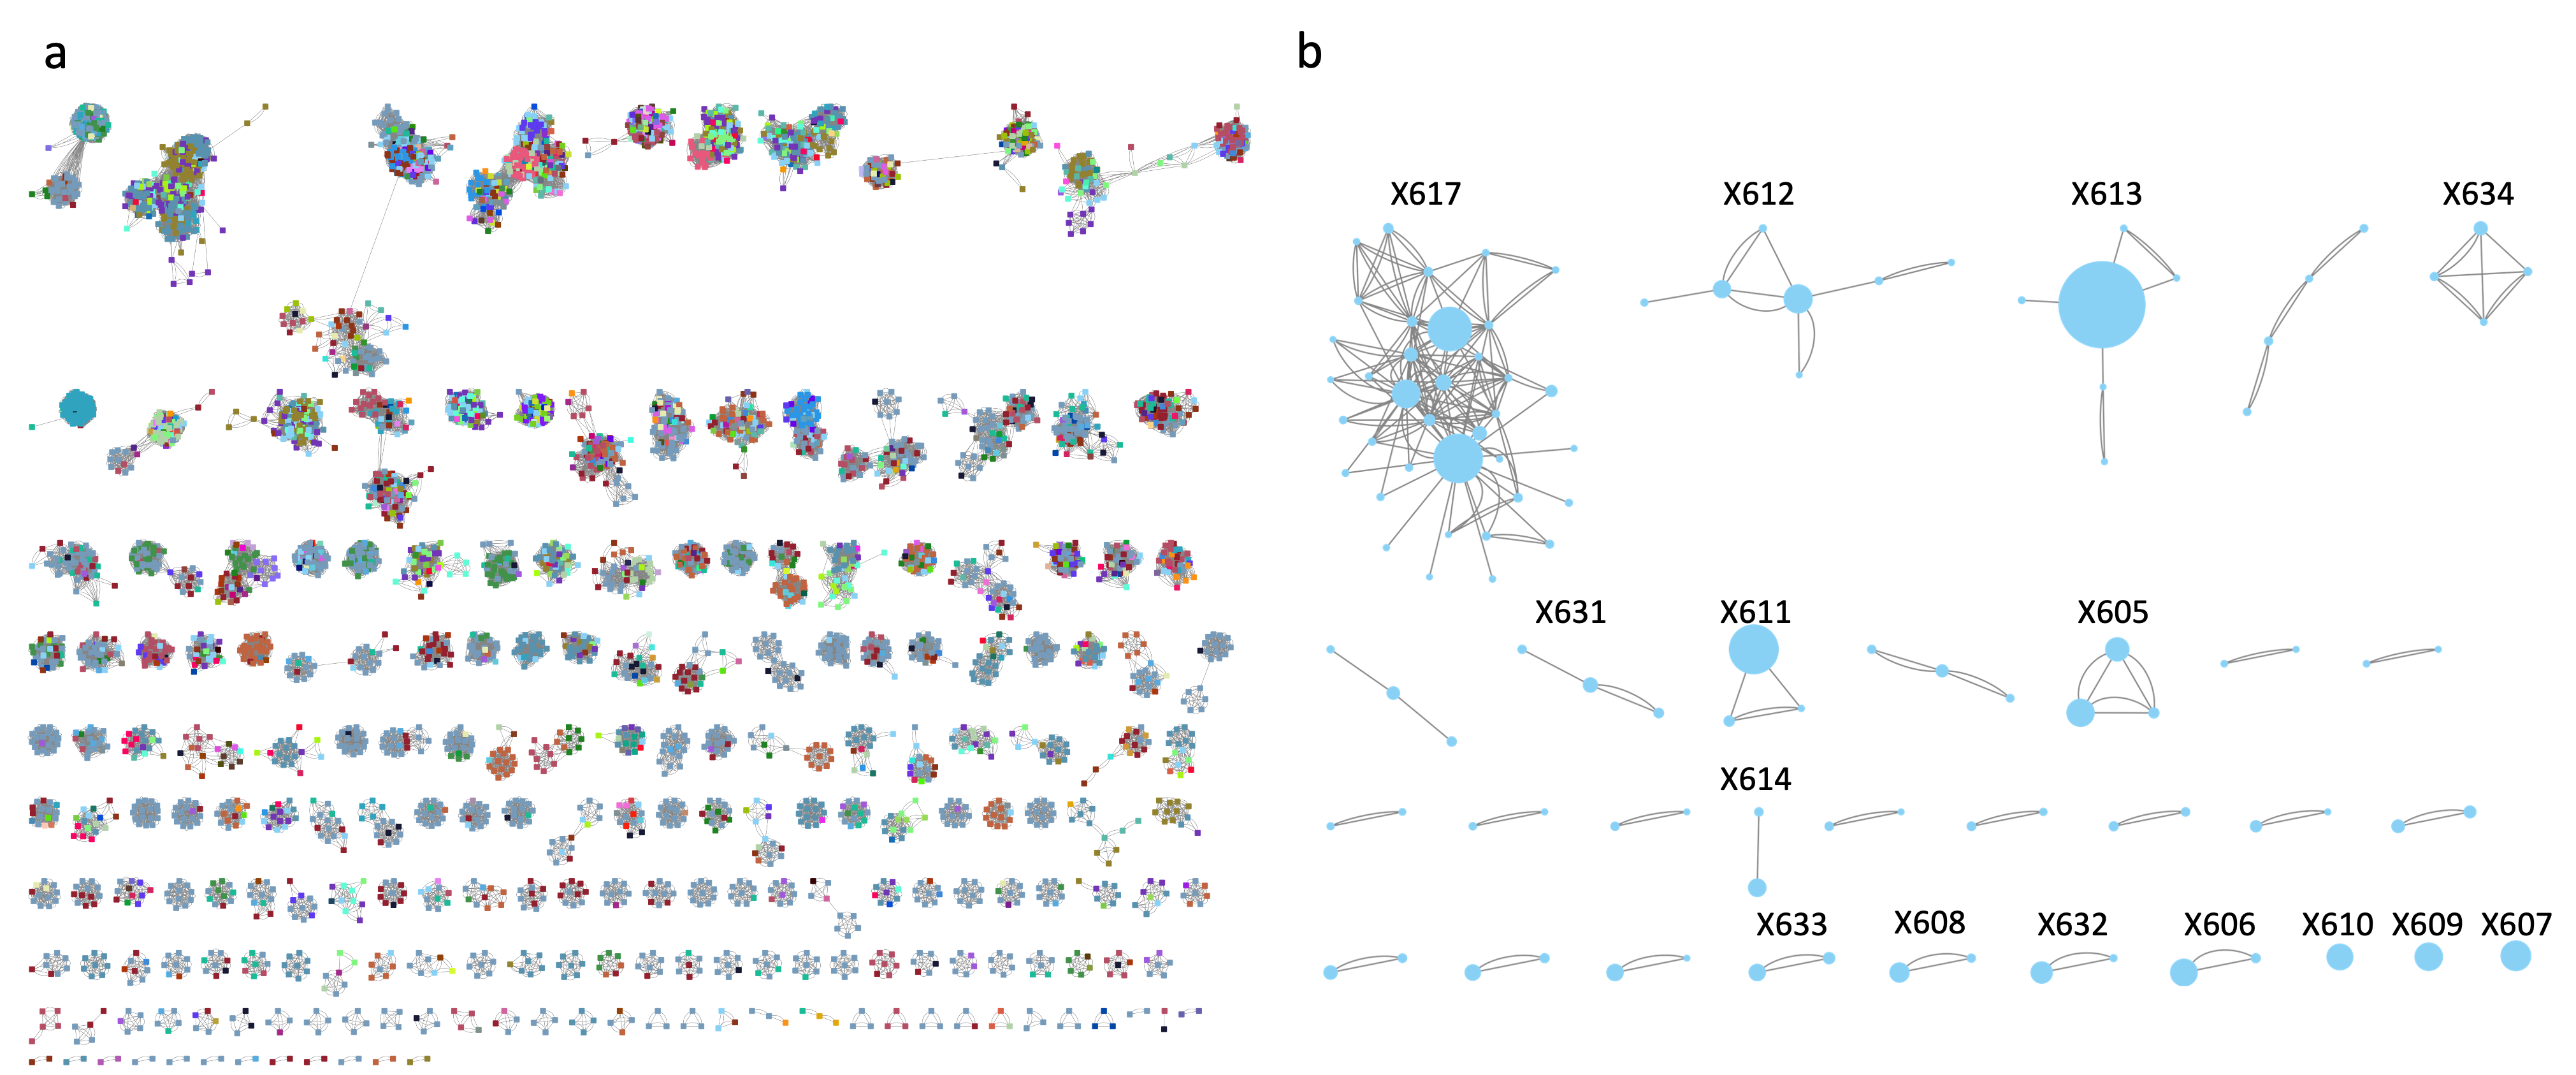
\includegraphics[width=\textwidth]{figures/network-figure.png}
    \caption{O-Pol clustering. a) SSN network. b) HHblits network.}
    \label{fig:wzy-clustering}
\end{figure}

\begin{figure}
    \centering
    \includegraphics{}
    \caption{Garry's heatmap}
    \label{fig:sugar-heatmap}
\end{figure}

\begin{figure}[htbp]
    \centering
    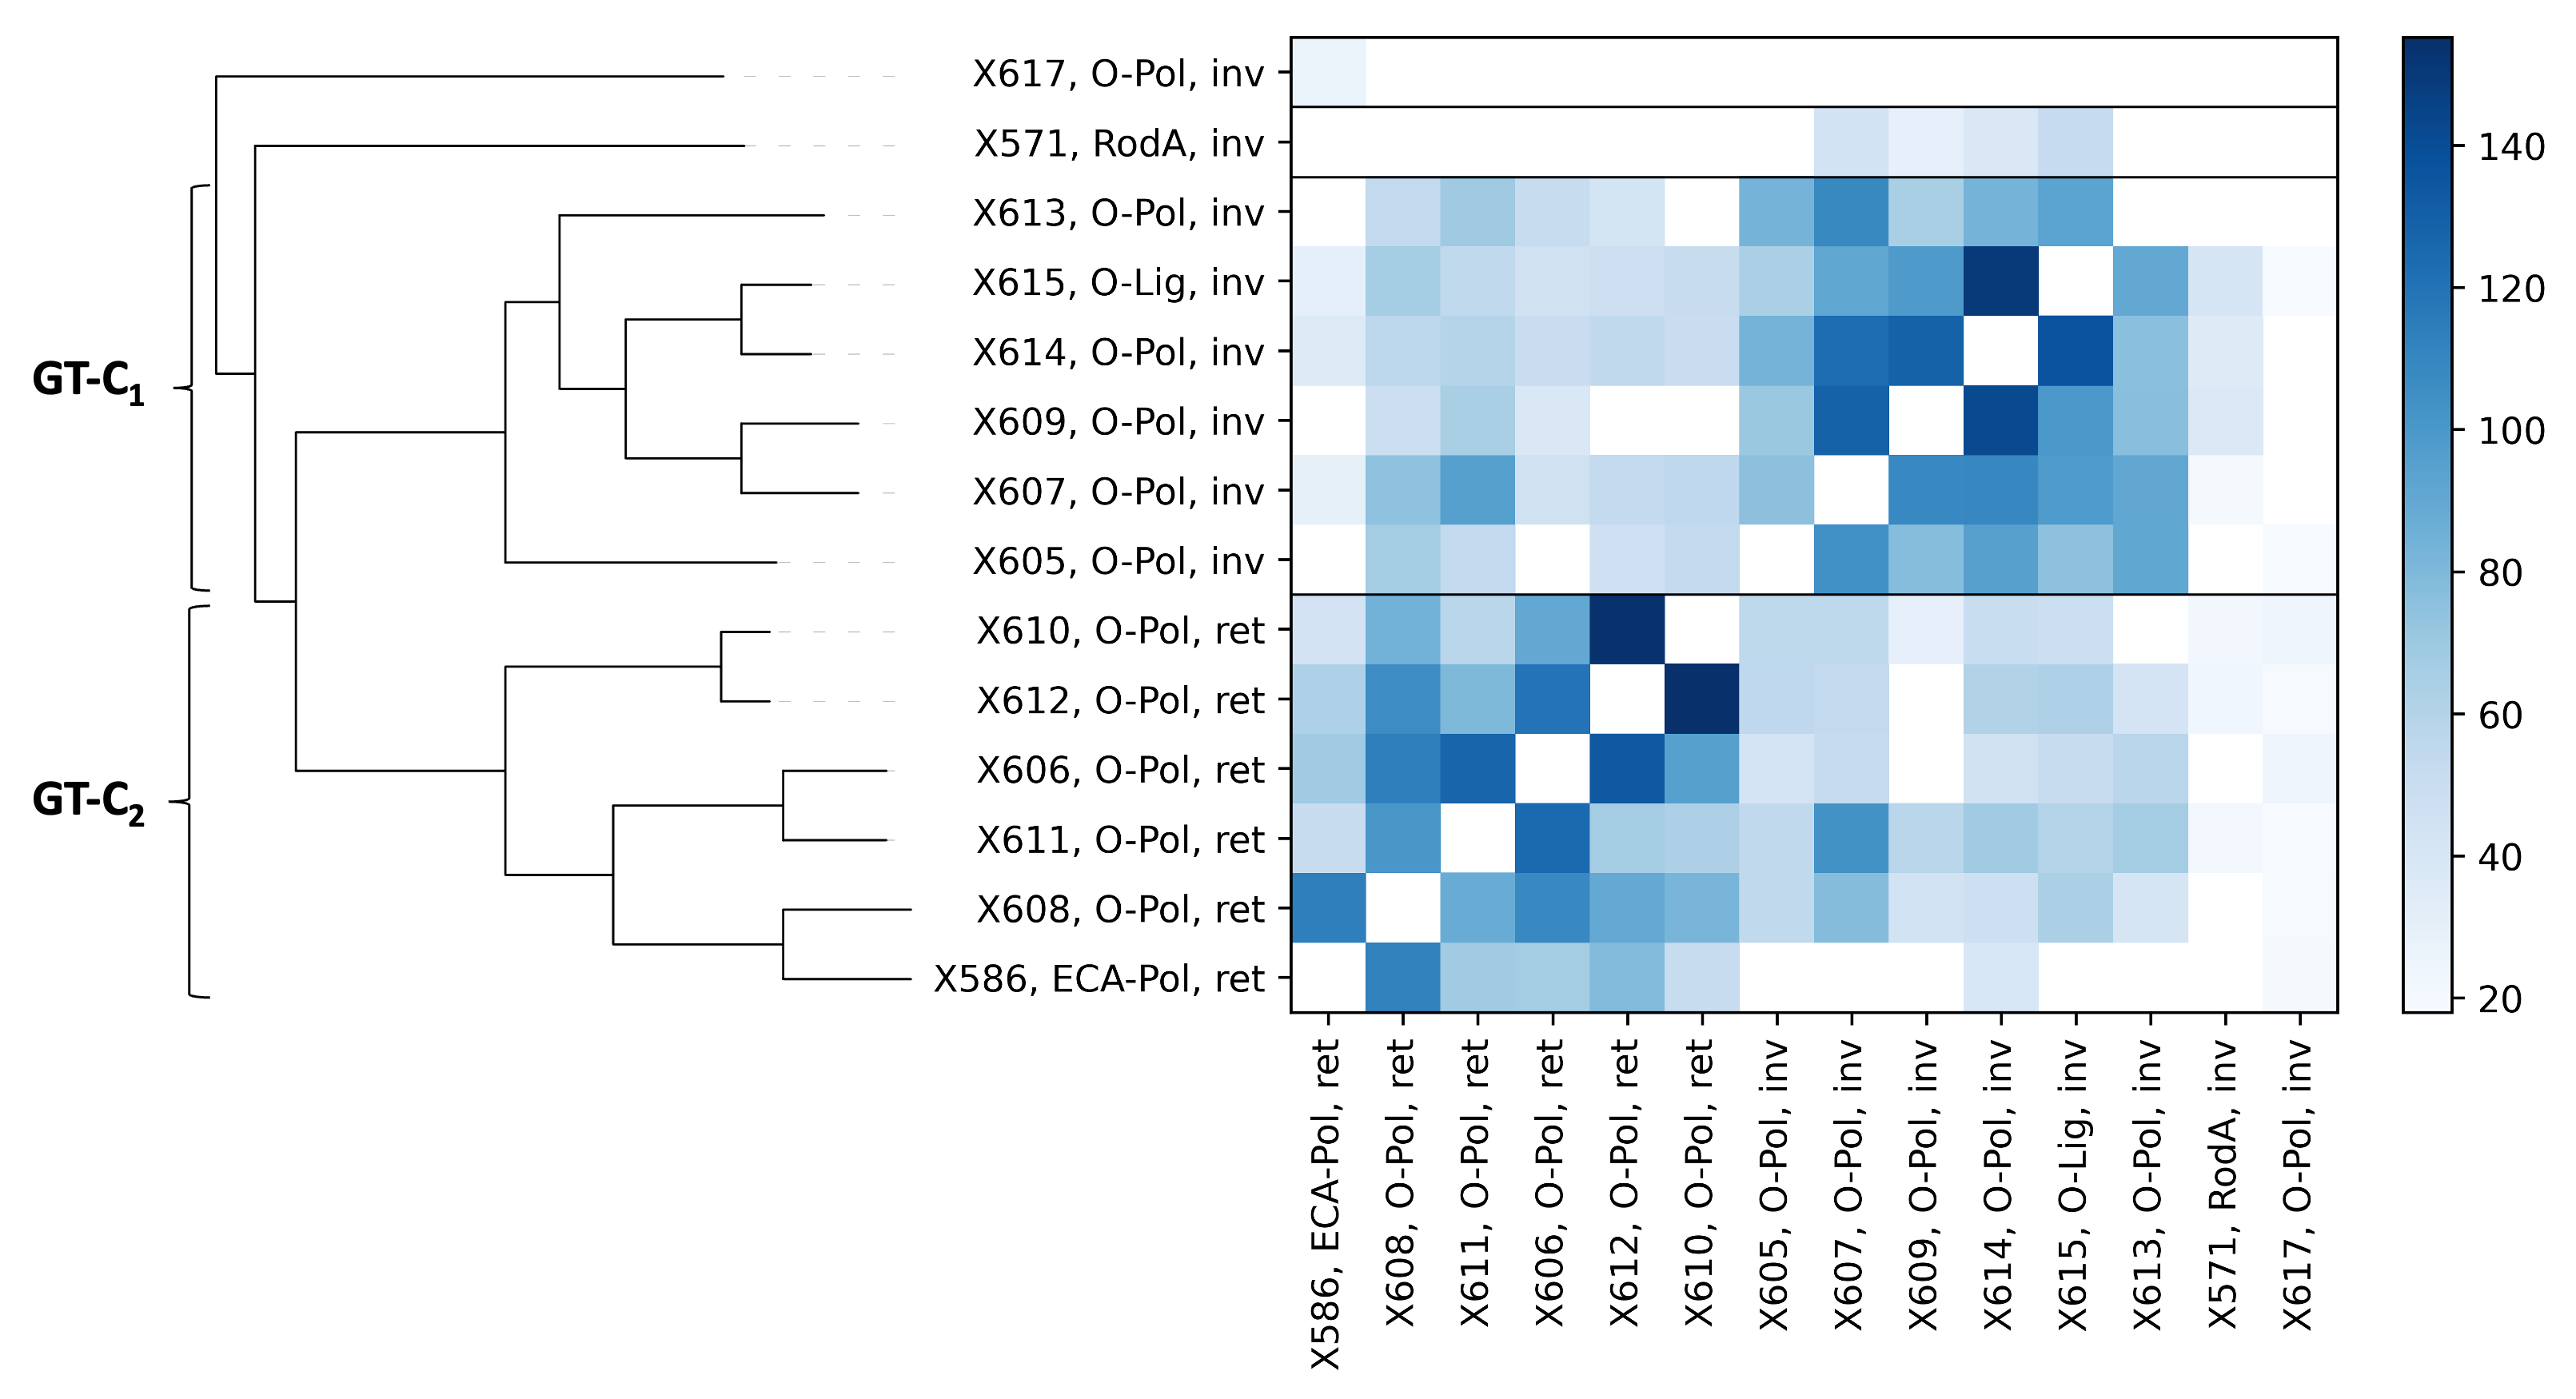
\includegraphics[width=.9\textwidth]{figures/heatmap_hhblits_edited.png}
    \caption{Heatmap of inter-family HHblits bit scores. The HHblits scores are shown on a color scale from white (low similarity score) to dark blue (high similarity score).}
    \label{fig:heatmap-hhblits}
\end{figure}

\begin{figure}[htbp]
    \centering
    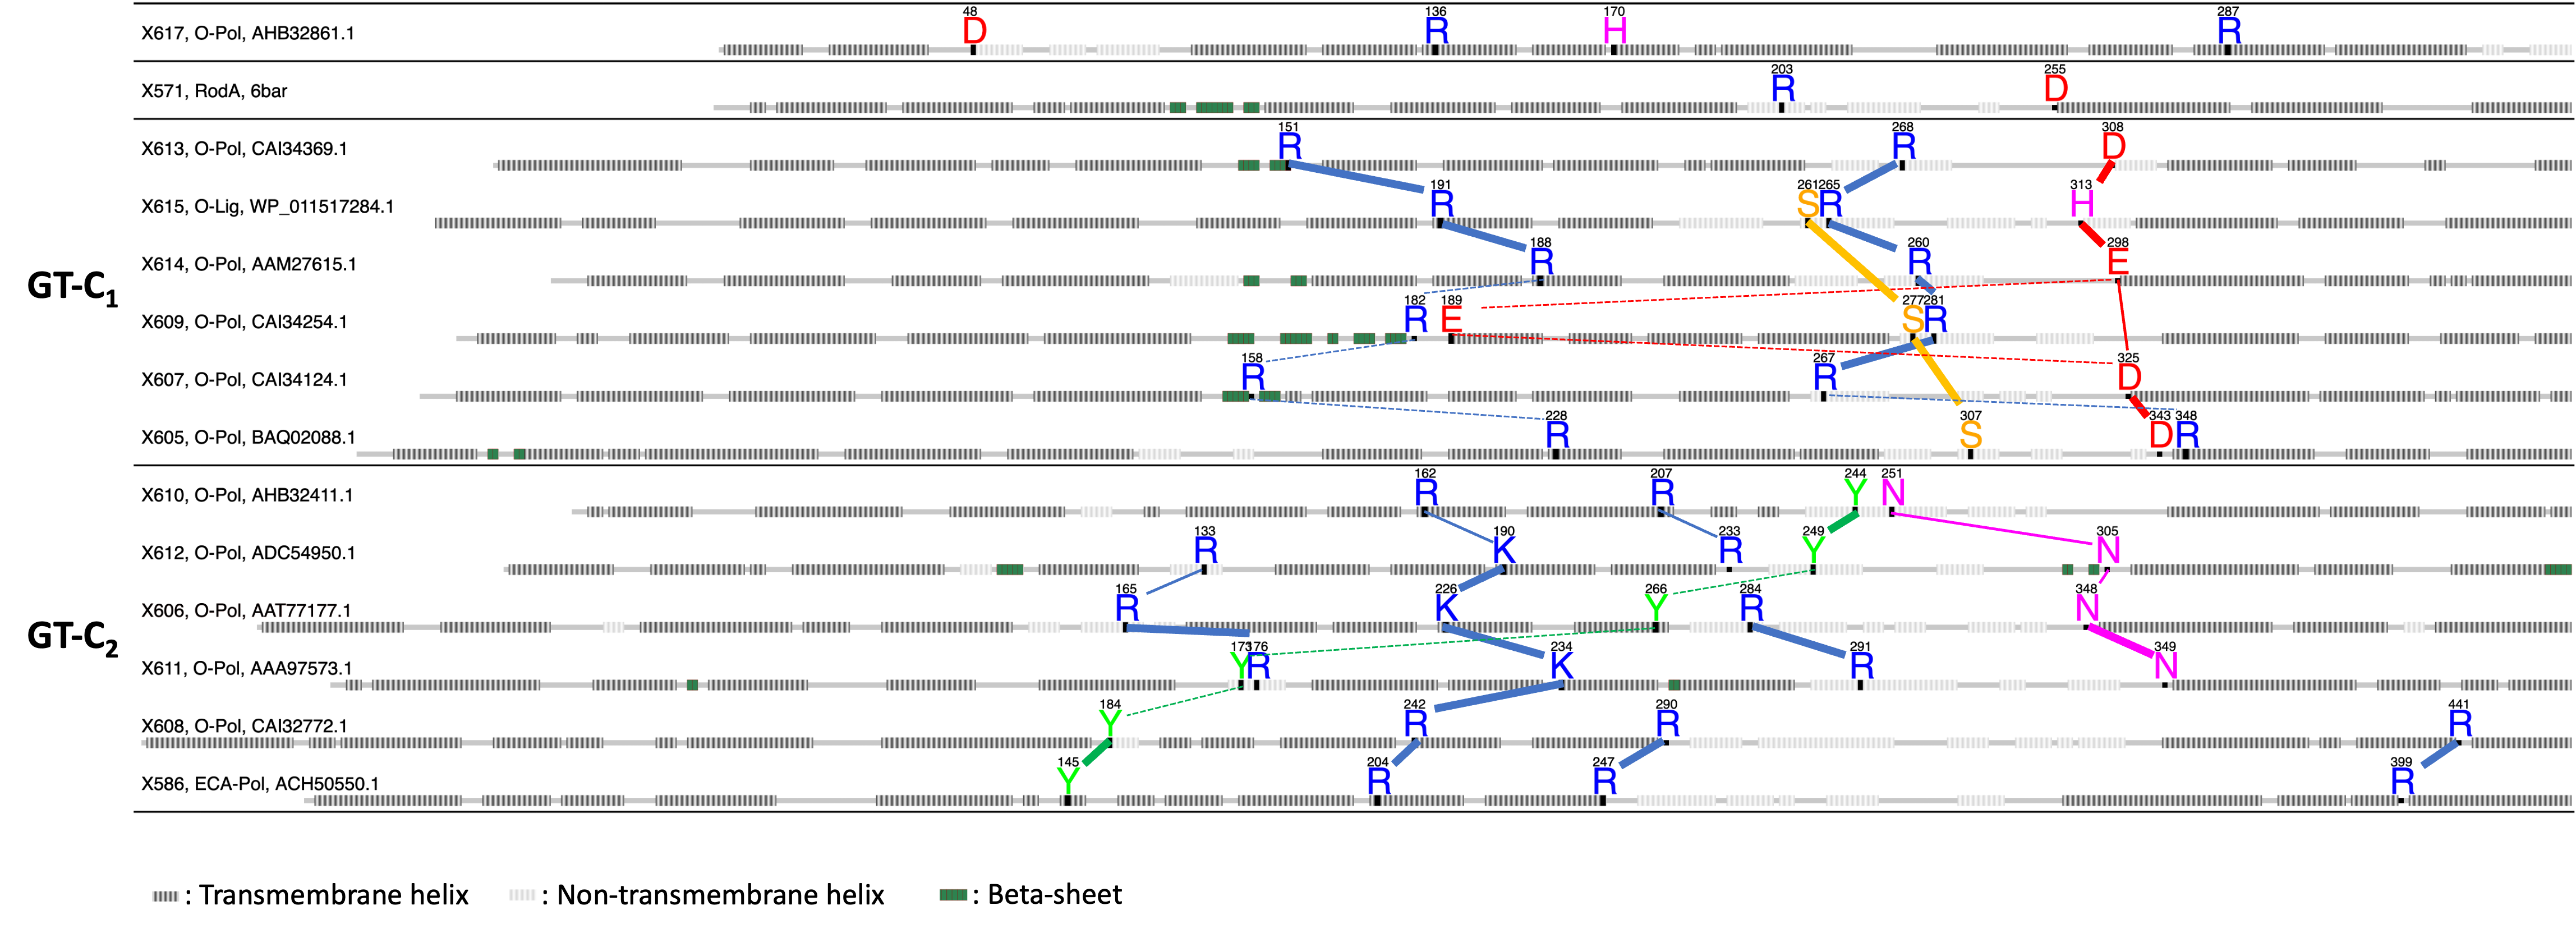
\includegraphics[width=\textwidth]{figures/architecture-comparison.png}
    \caption{The conserved residues of each of the new CAZy family shown on representative sequences. Thick lines are shown between residues that align in HHblits. Thin lines are shown between residues that align structurally. Dashed lines are shown between residues that do not overlap completely, but take up the same space structurally.}
    \label{fig:architecture-comparison}
\end{figure}

\begin{figure}
    \centering
    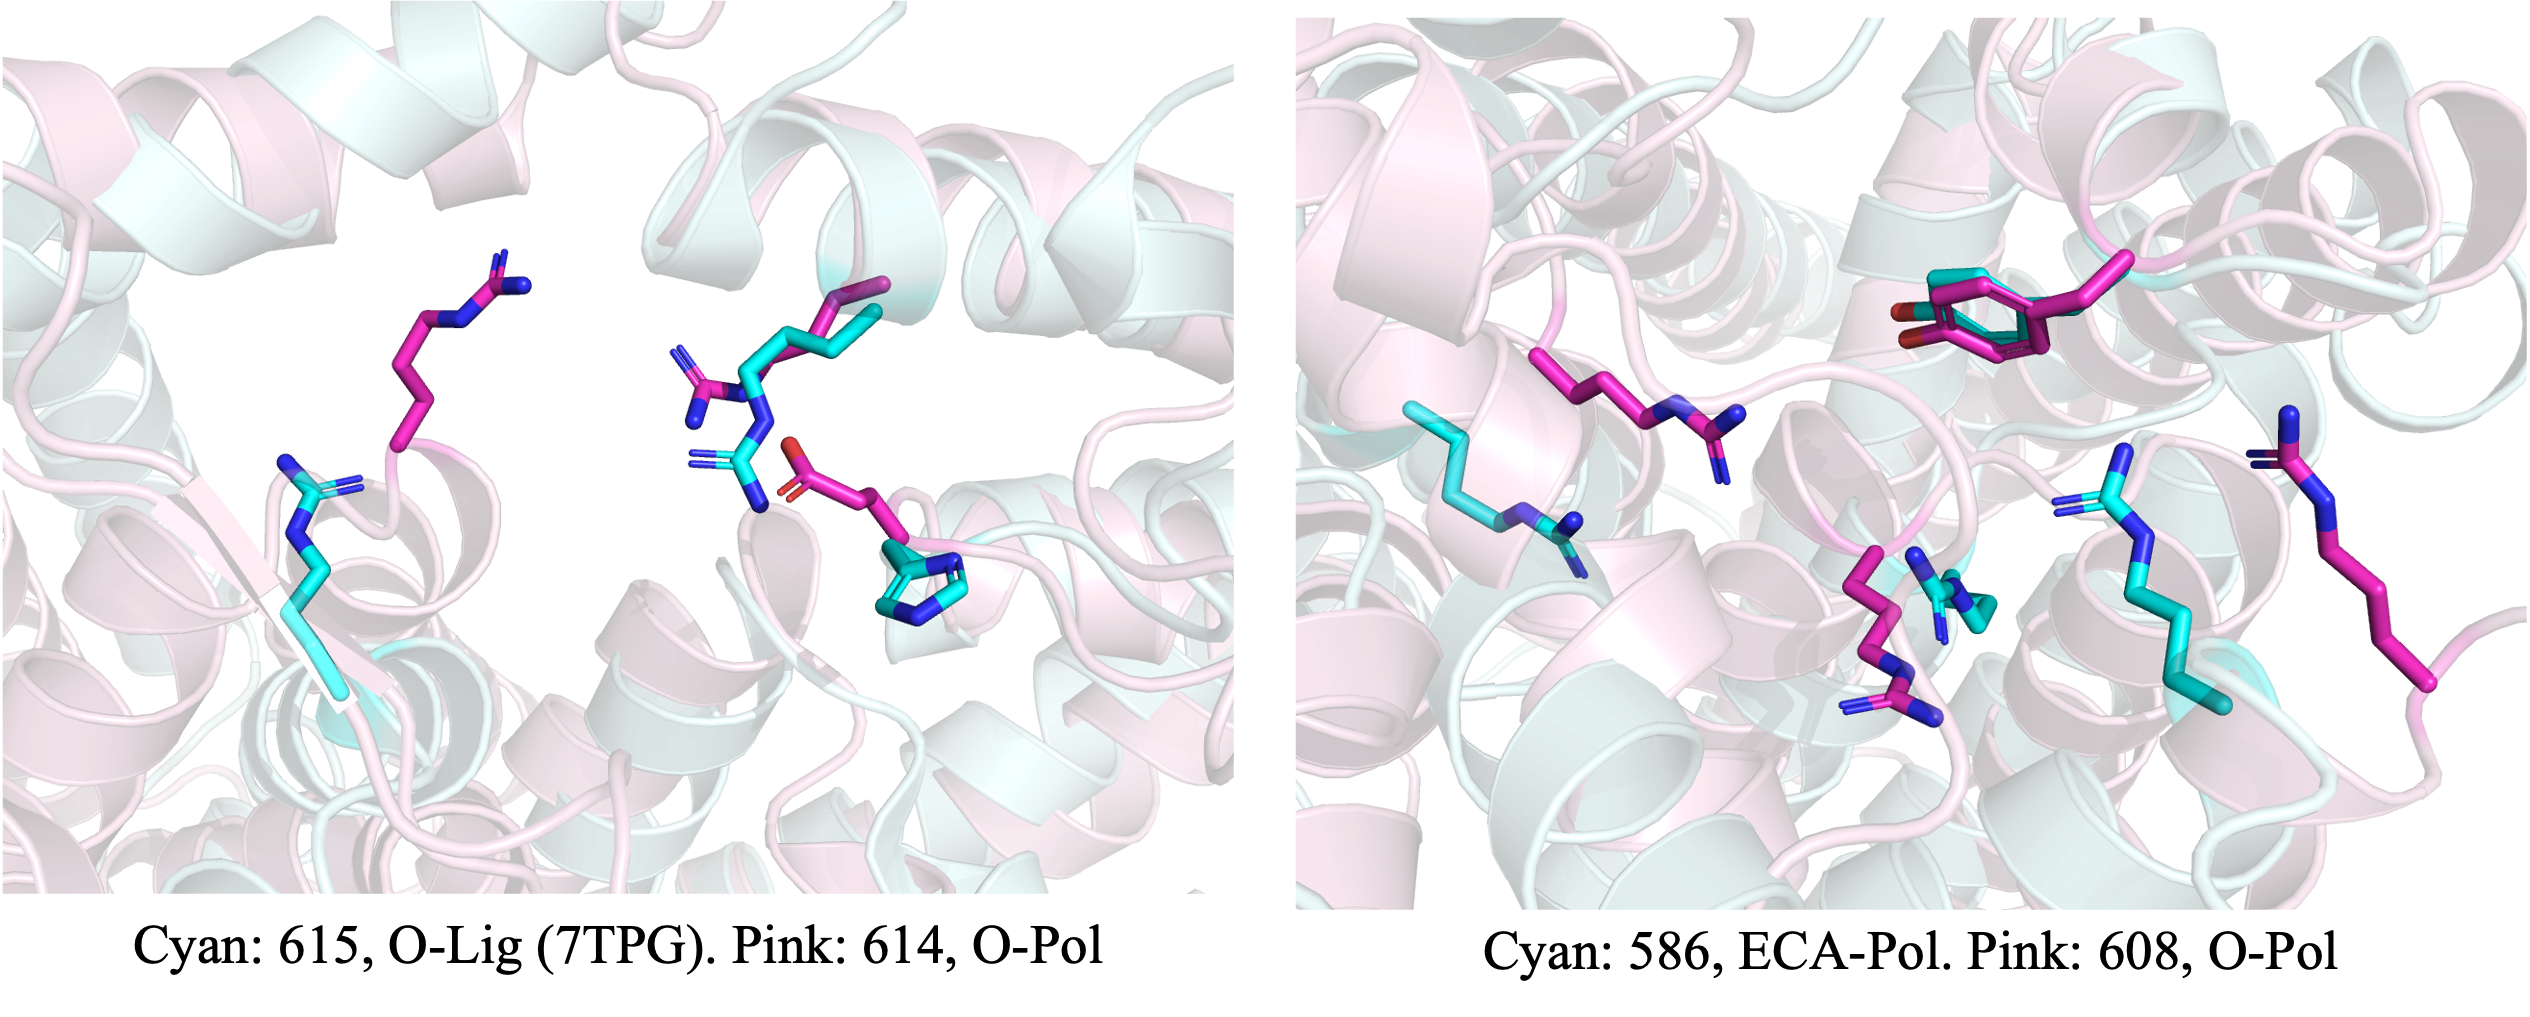
\includegraphics[width=.9\textwidth]{figures/structural-alignments2.png}
    \caption{Structural superimposition of different families.}
    \label{fig:structural_alignments}
\end{figure}

\clearpage

\section{Supplementary material}

\begin{figure}[htbp]
    \centering
    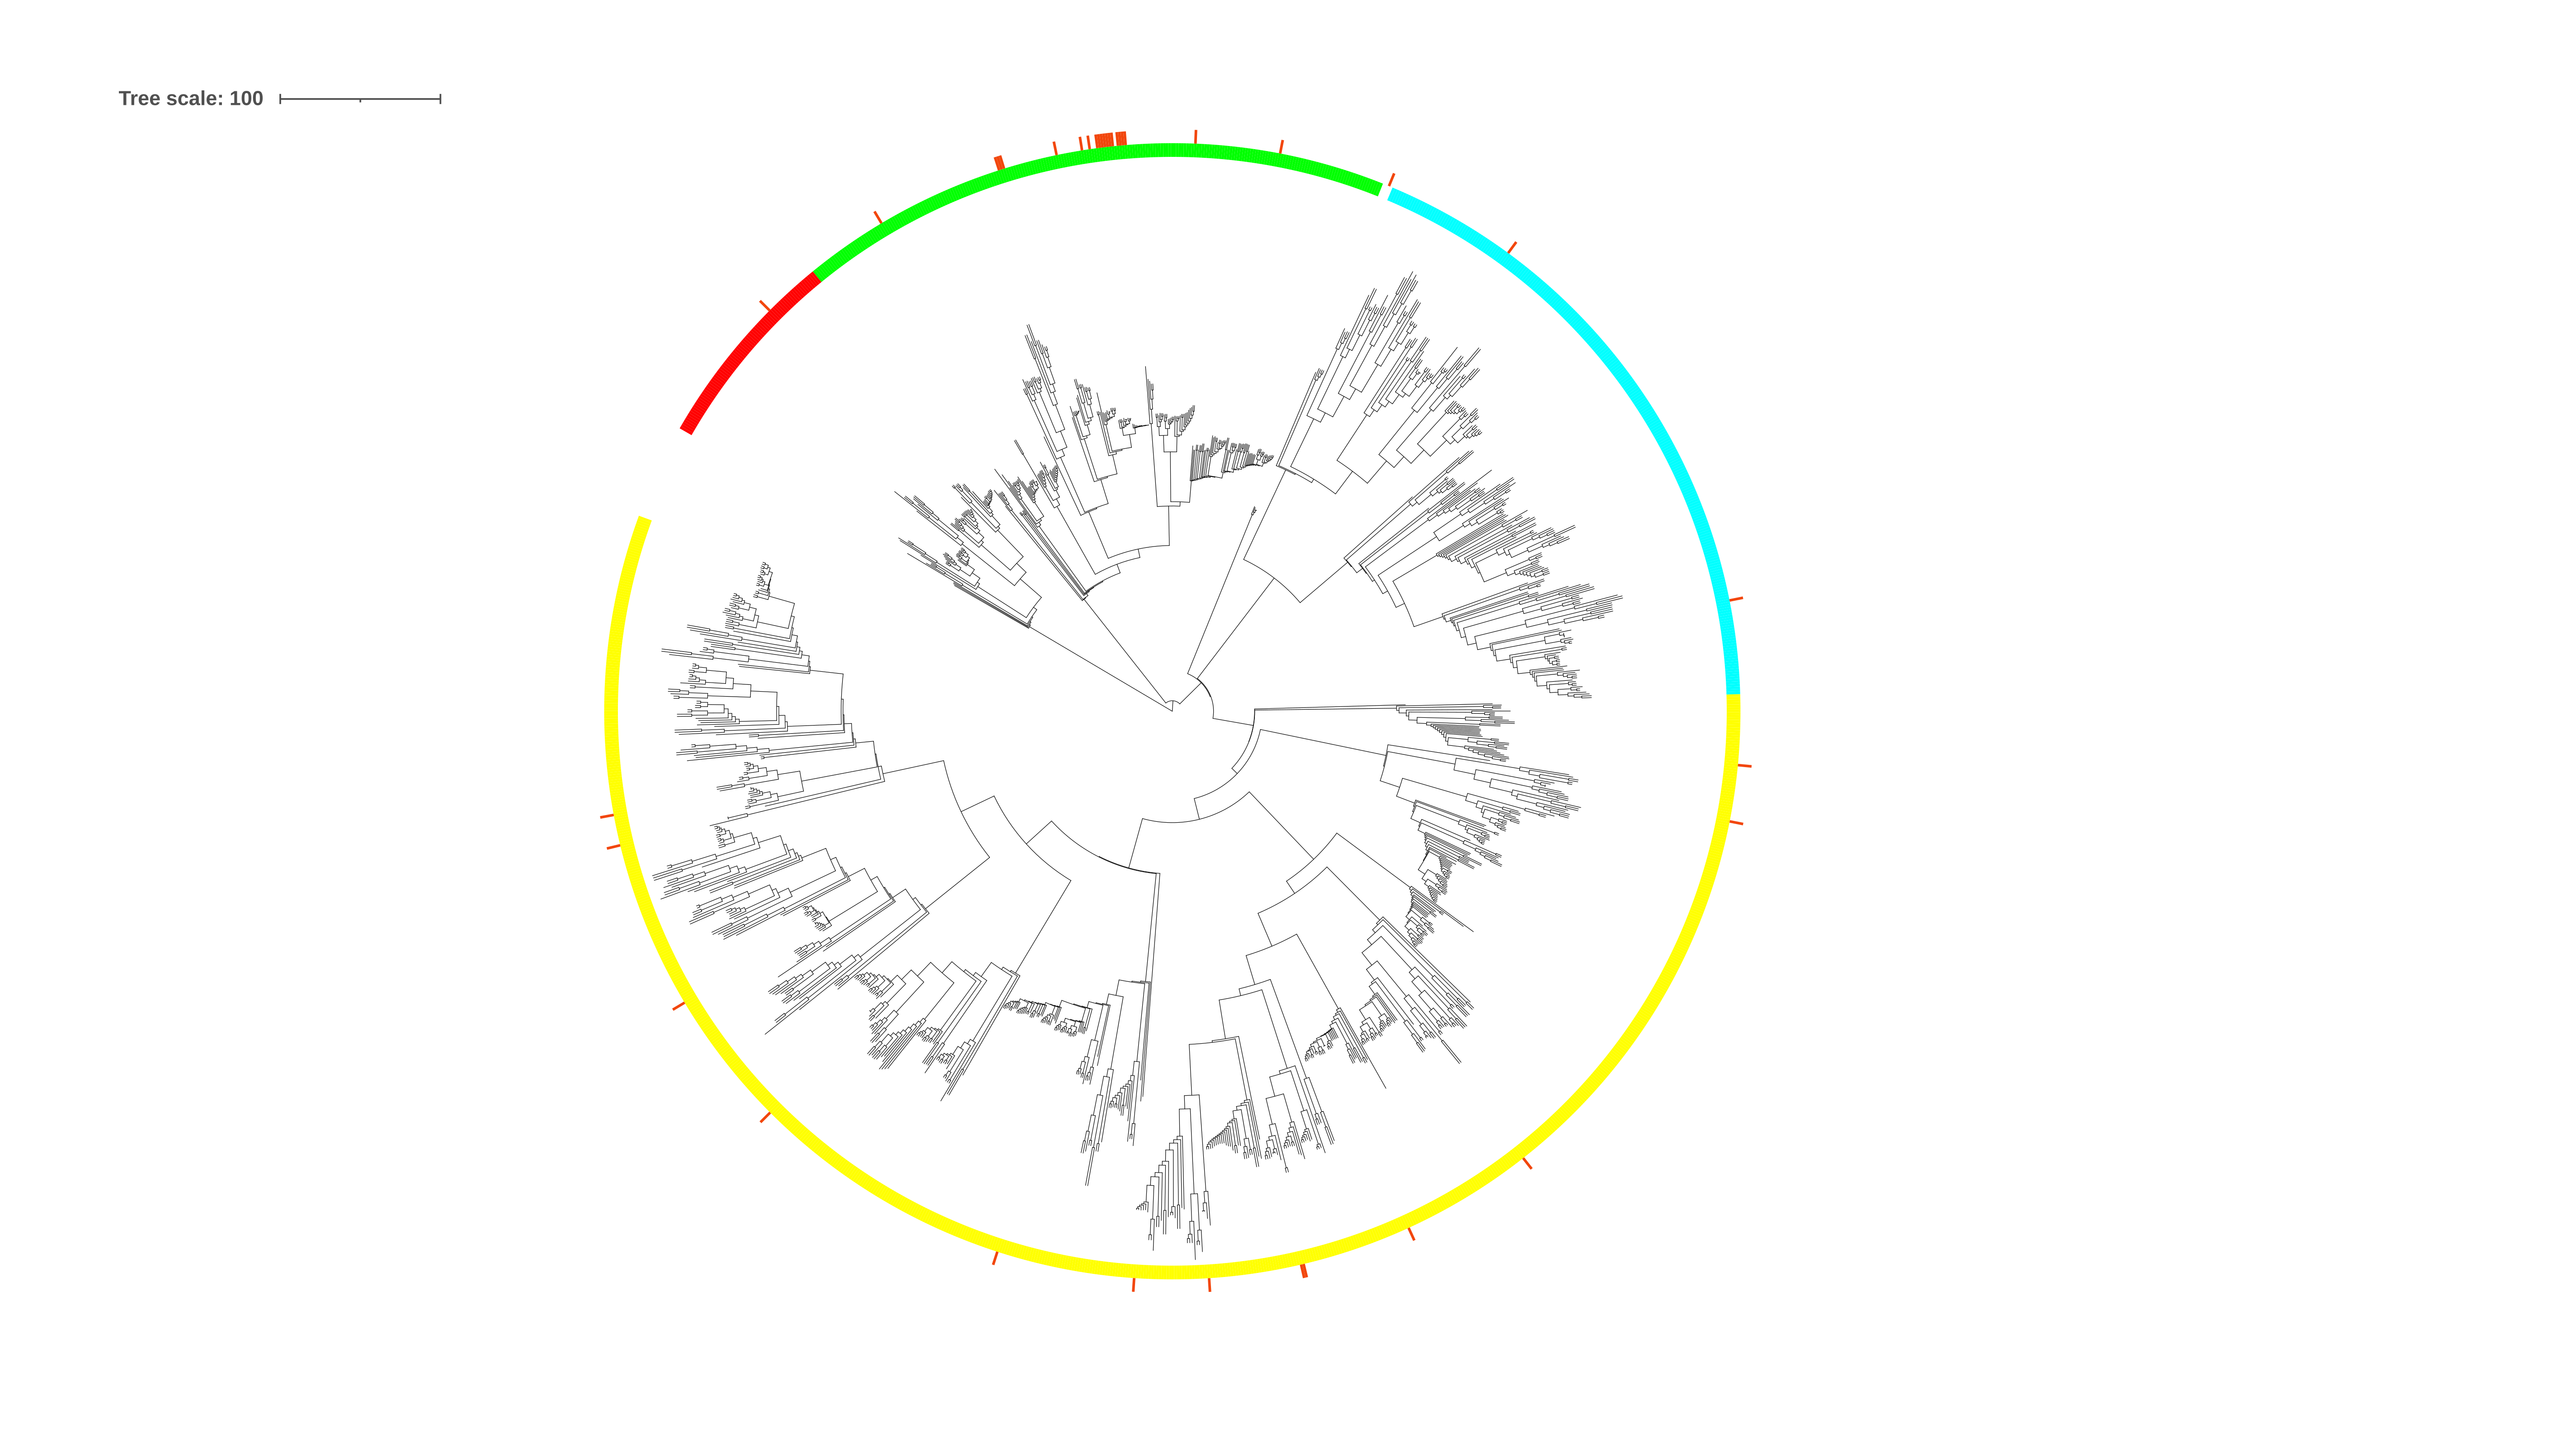
\includegraphics[width=\textwidth]{figures/o-lig-tree.png}
    \caption{Aclust tree of O-Lig sequence space}
    \label{fig:o-lig-tree}
\end{figure}
%https://itol.embl.de/tree/1923890169346361673971155#

\begin{figure}
    \centering
    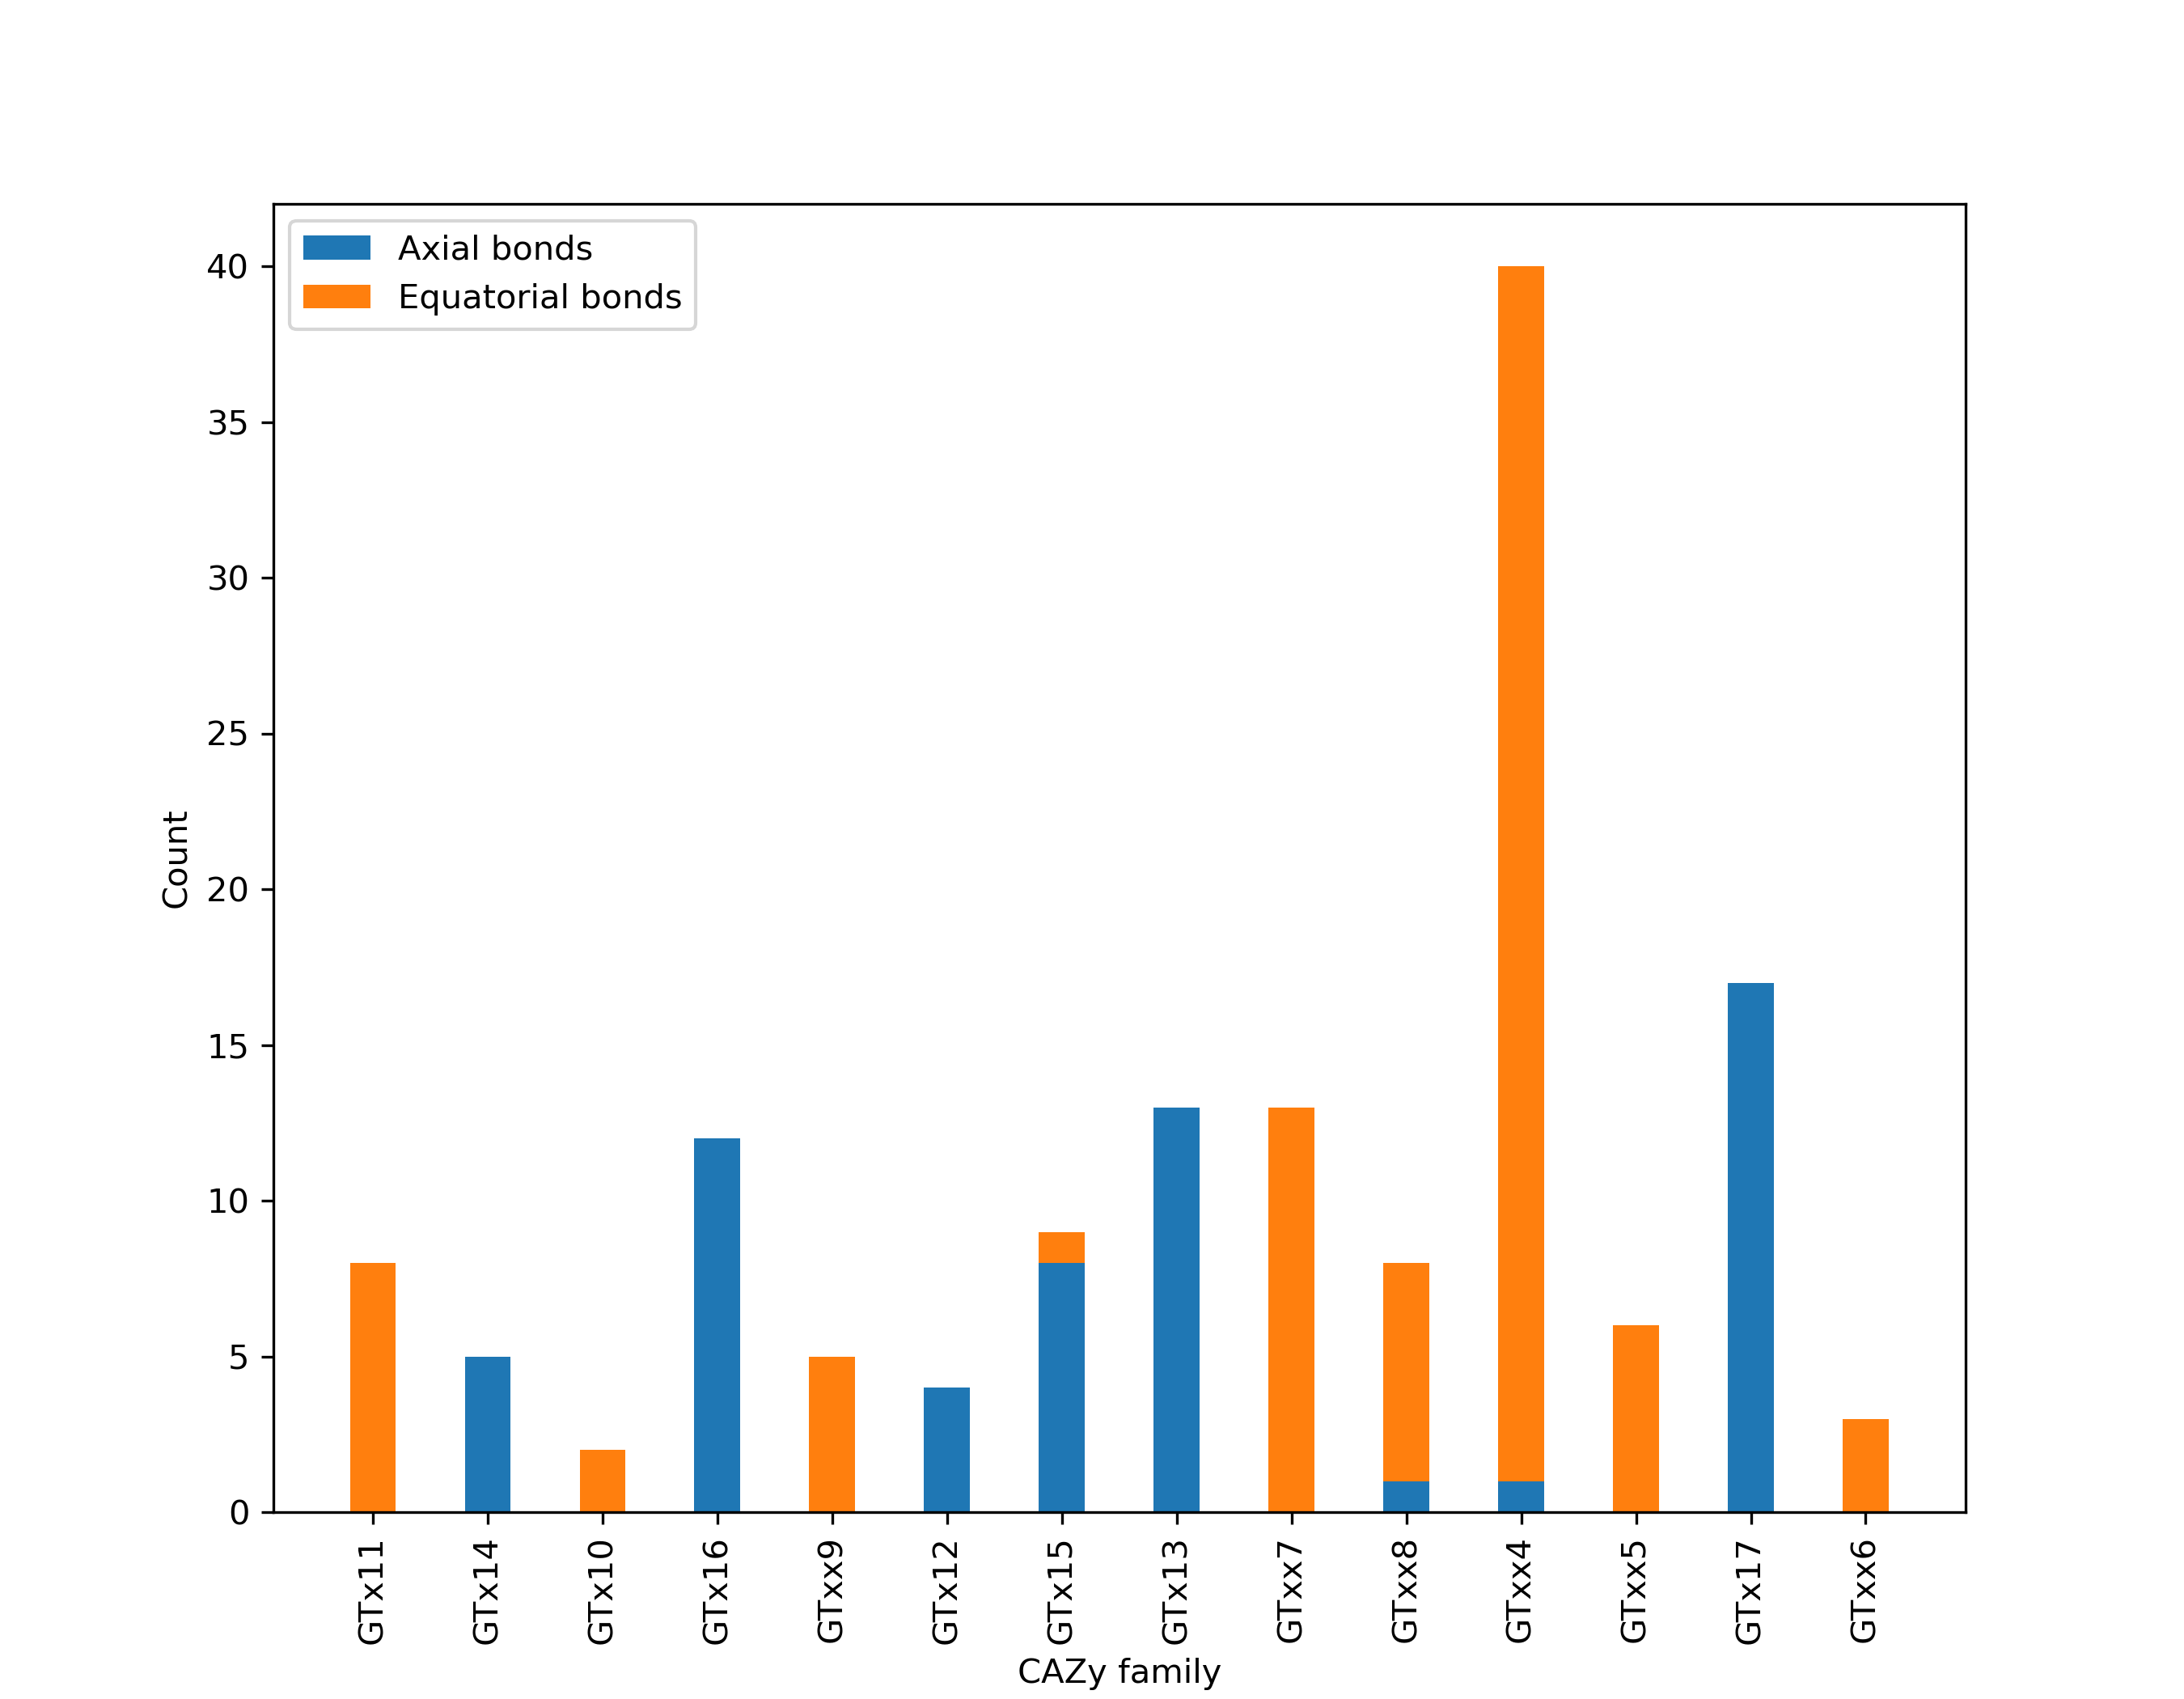
\includegraphics[width=0.9\textwidth]{figures/stereochemistry-final.png}
    \caption{Stereochemistry of the bond made by the polymerase in each family (will be remade when we have the final list of members)}
    \label{fig:stereochemistry-barplot}
\end{figure}

\begin{figure}[htbp]
    \centering
    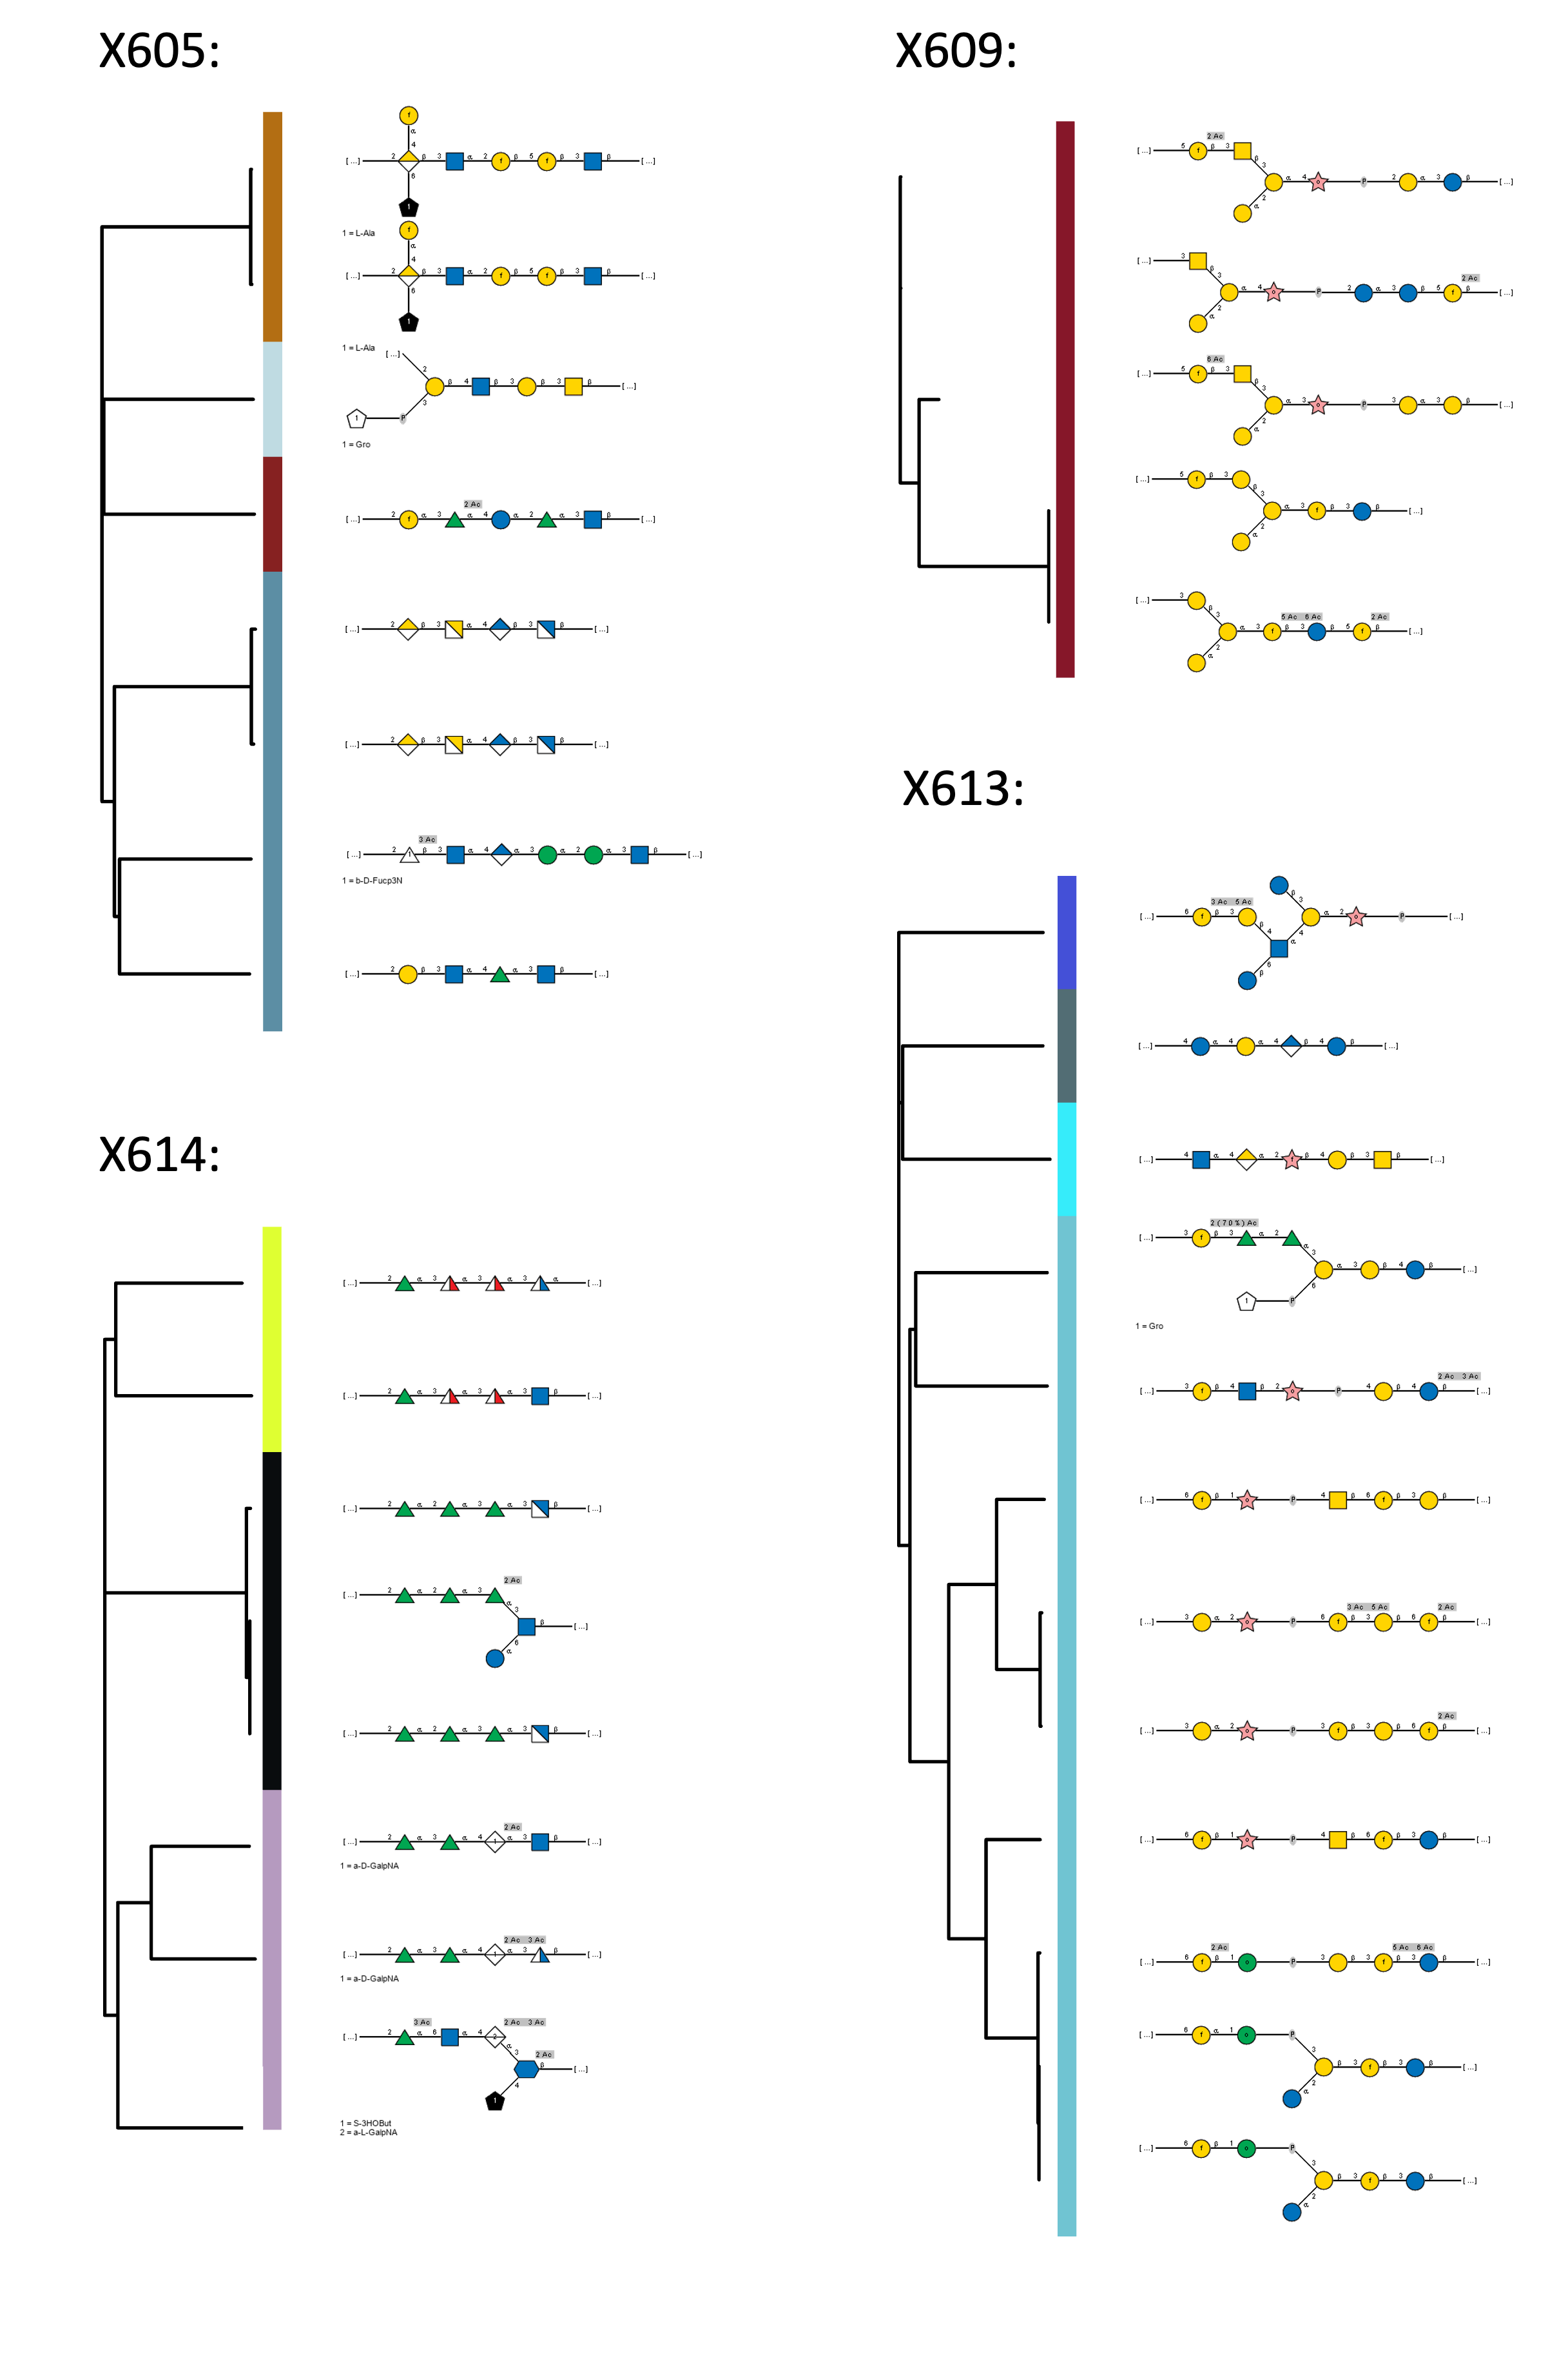
\includegraphics[width=.95\textwidth]{figures/sugar-tree-GTC2.png}
    \caption{Phylogenetic trees of the O-Pols from clan GT-C\textsubscript{1} with structures of the corresponding sugar repeat units.}
    \label{fig:sugar-tree-GTC2}
\end{figure}

\begin{figure}[htbp]
    \centering
    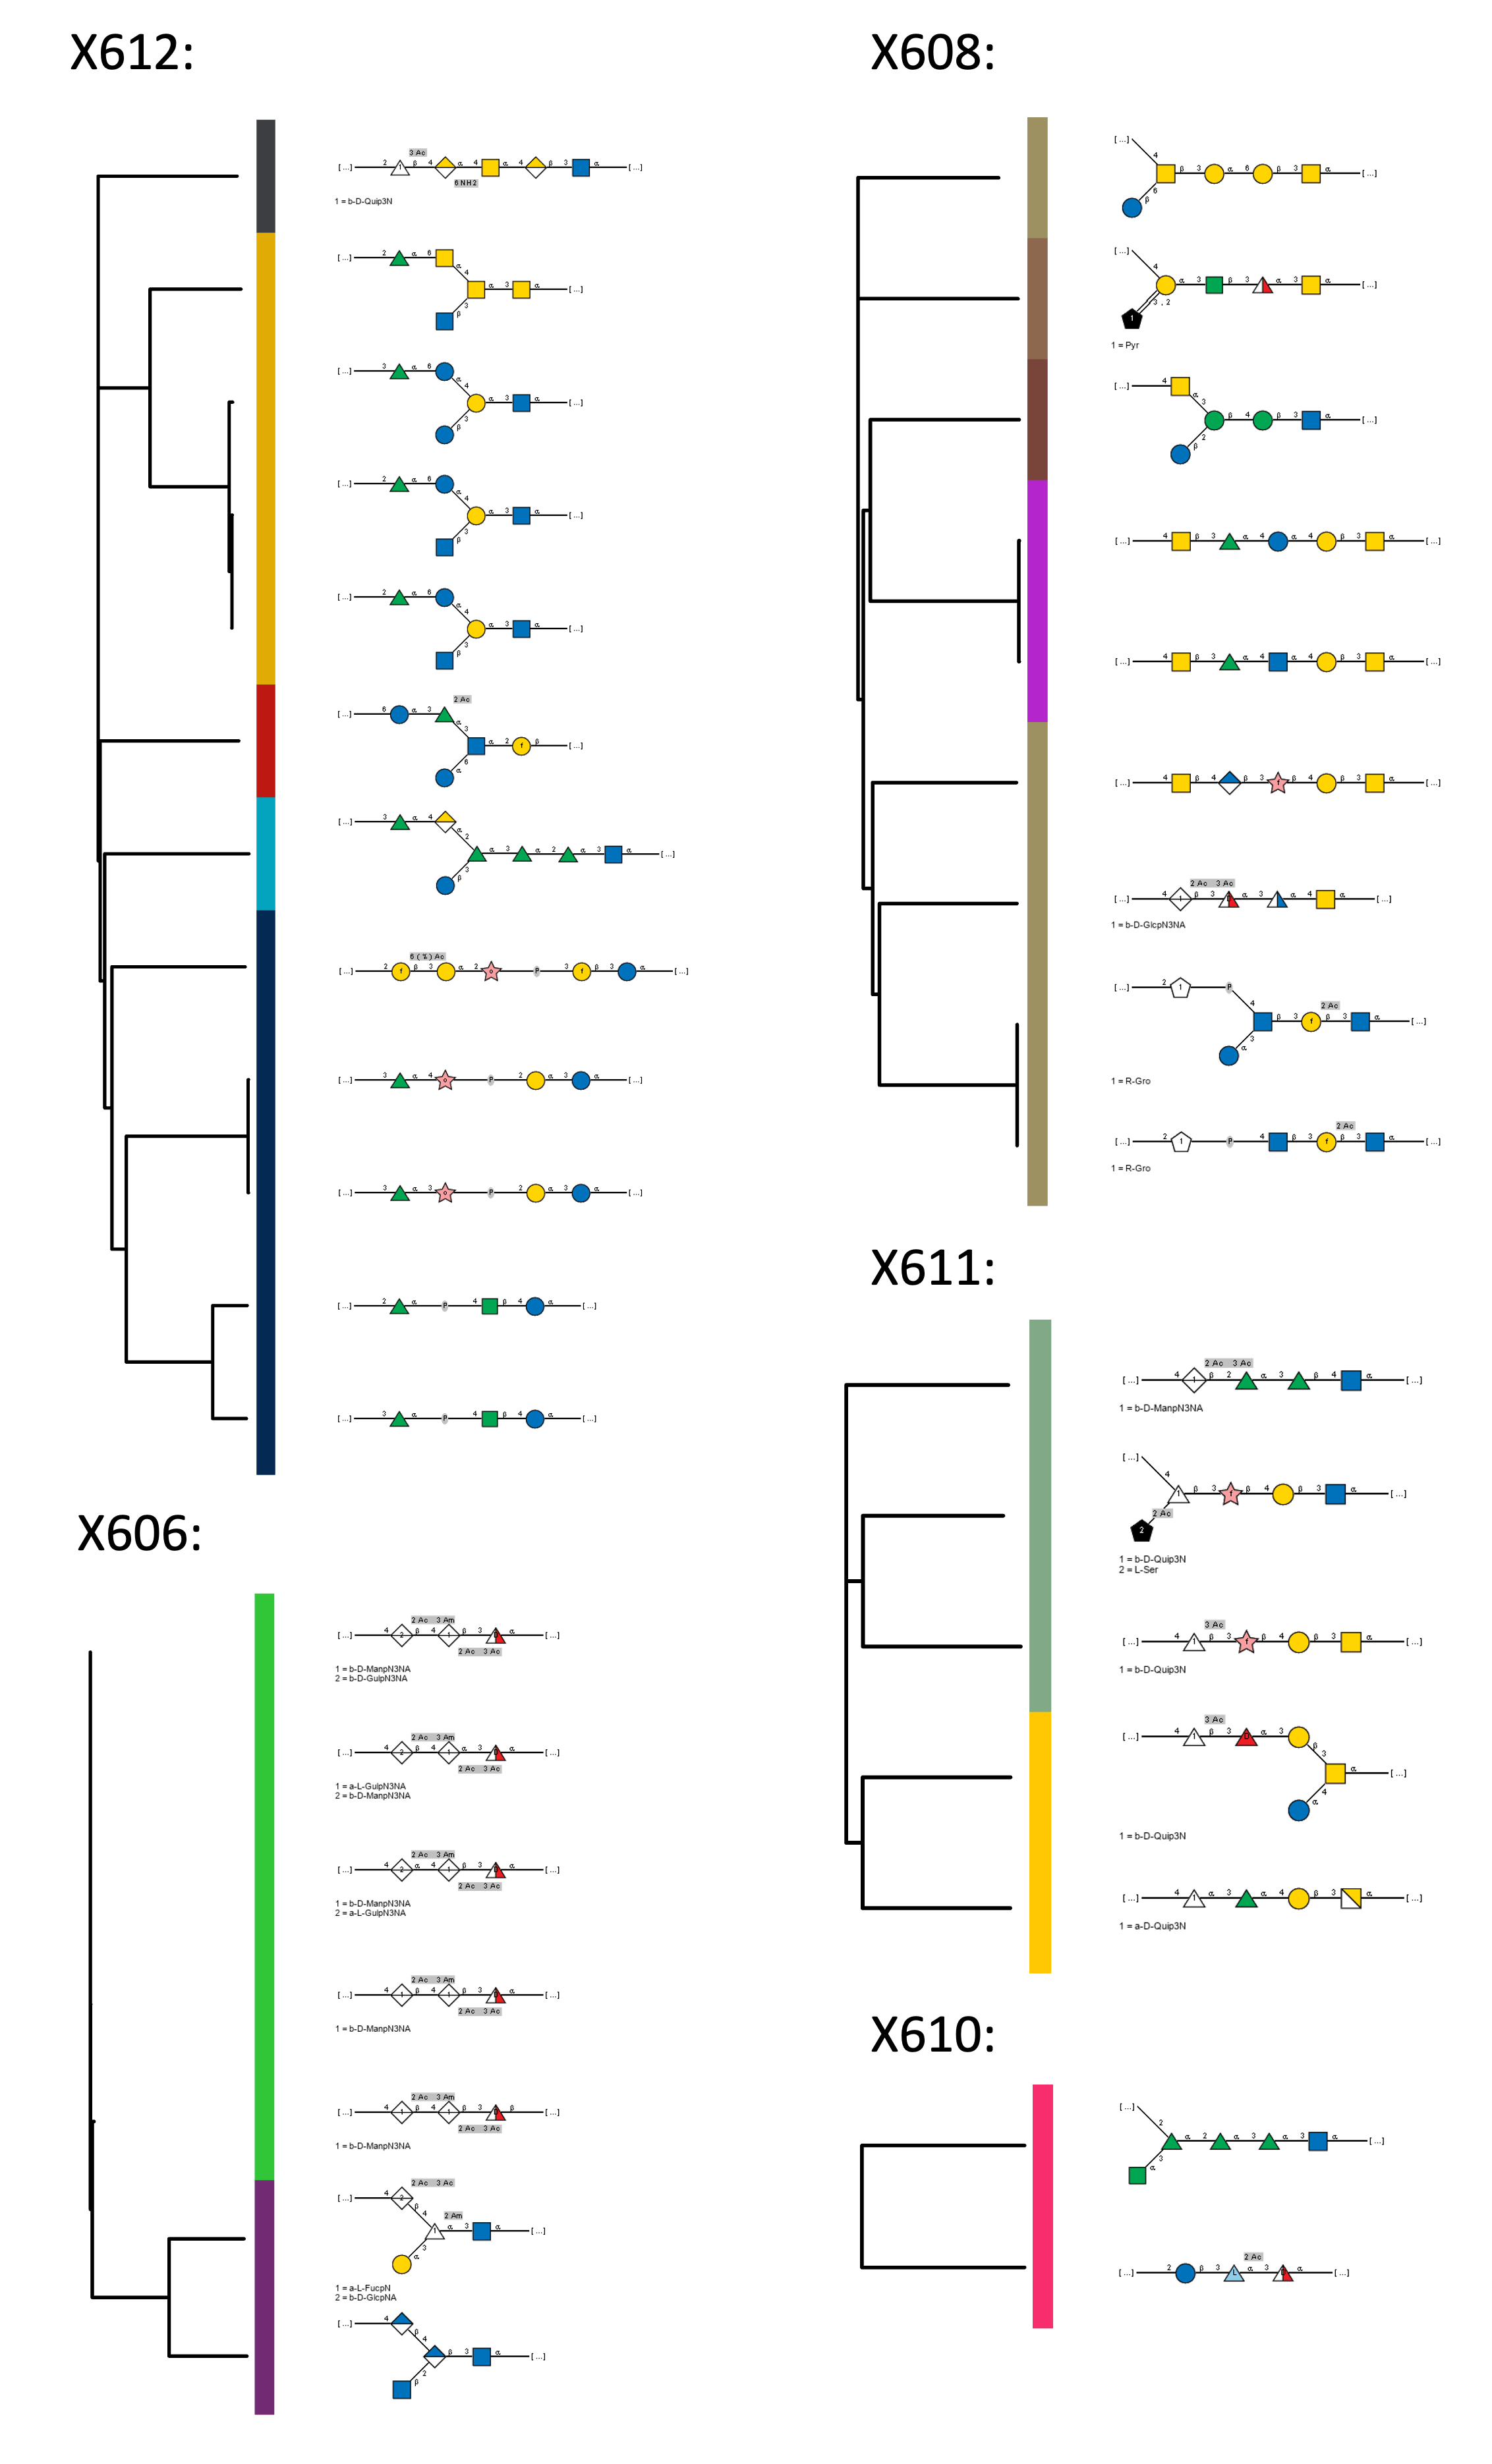
\includegraphics[width=.85\textwidth]{figures/sugar-tree-GTC3.png}
    \caption{Phylogenetic trees of the O-Pols from clan GT-C\textsubscript{2} with structures of the corresponding sugar repeat units.}
    \label{fig:sugar-tree-GTC3}
\end{figure}

\begin{figure}[htbp]
    \centering
    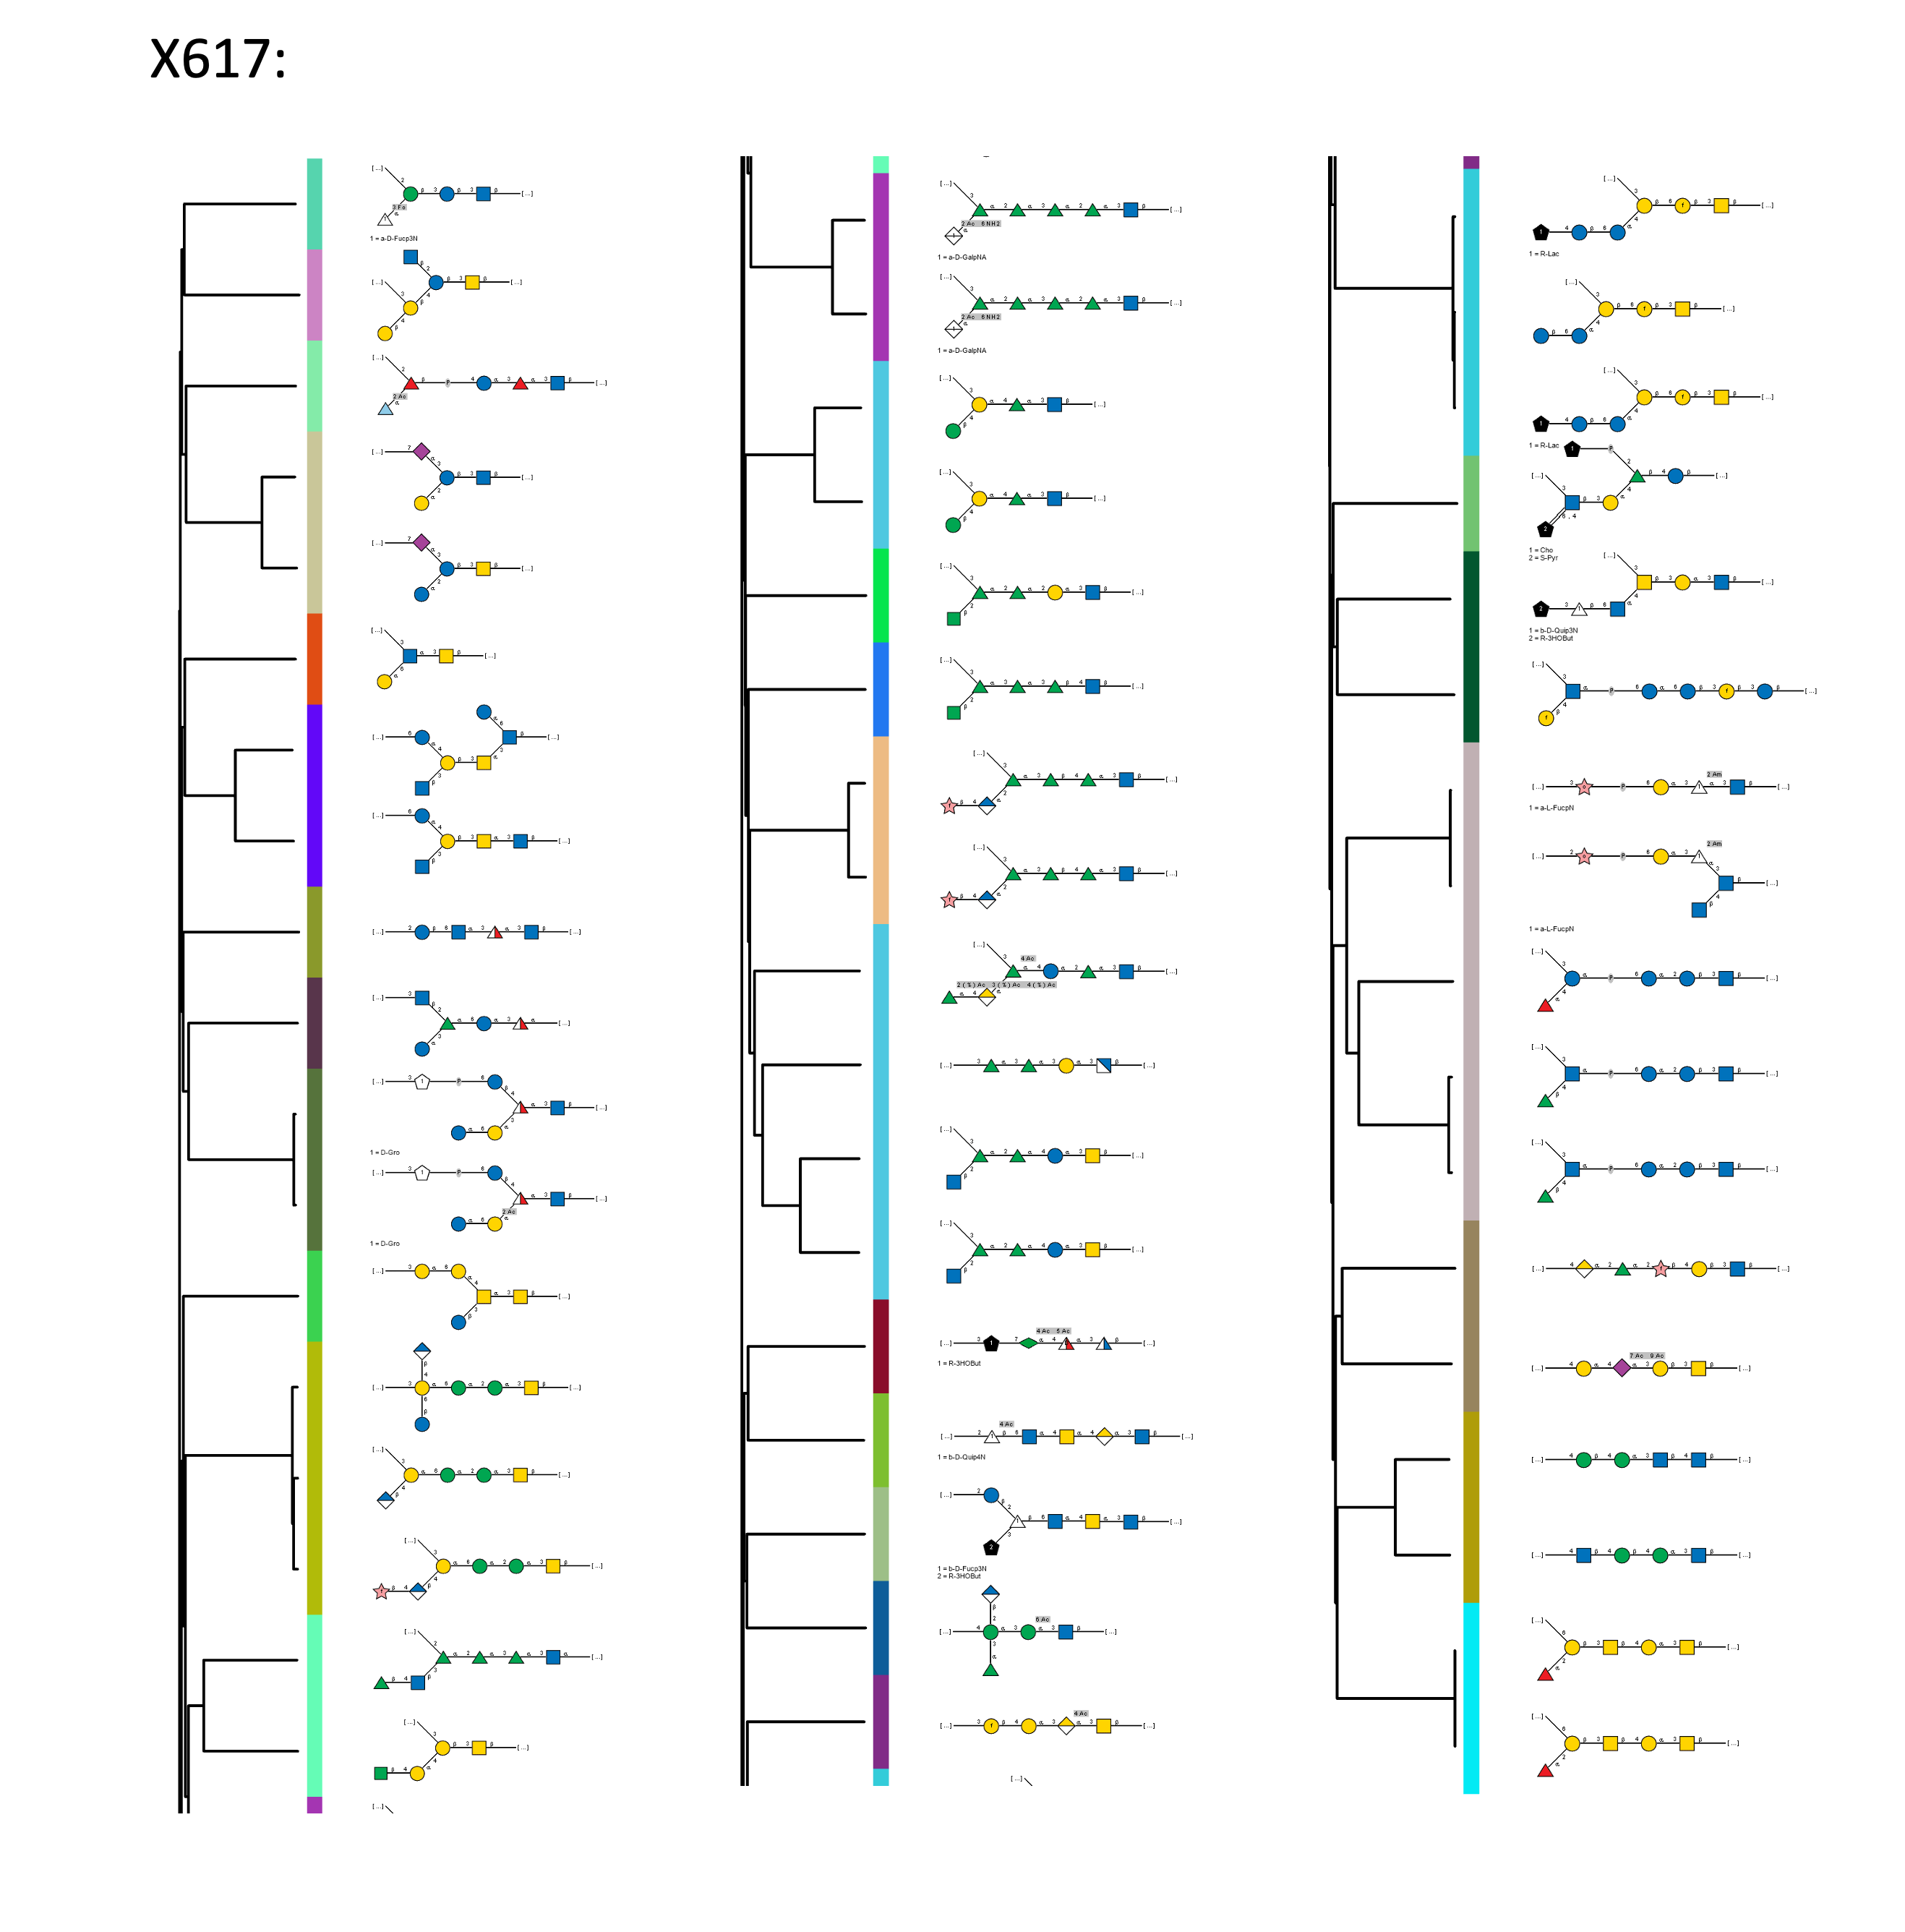
\includegraphics[width=\textwidth]{figures/sugar-tree-GTC4.png}
    \caption{Phylogenetic trees of the O-Pols from clan GT-C\textsubscript{3} with structures of the corresponding sugar repeat units.}
    \label{fig:sugar-tree-GTC4}
\end{figure}

\clearpage

\section{Scratchpad}

\begin{figure}[htbp]
    \centering
    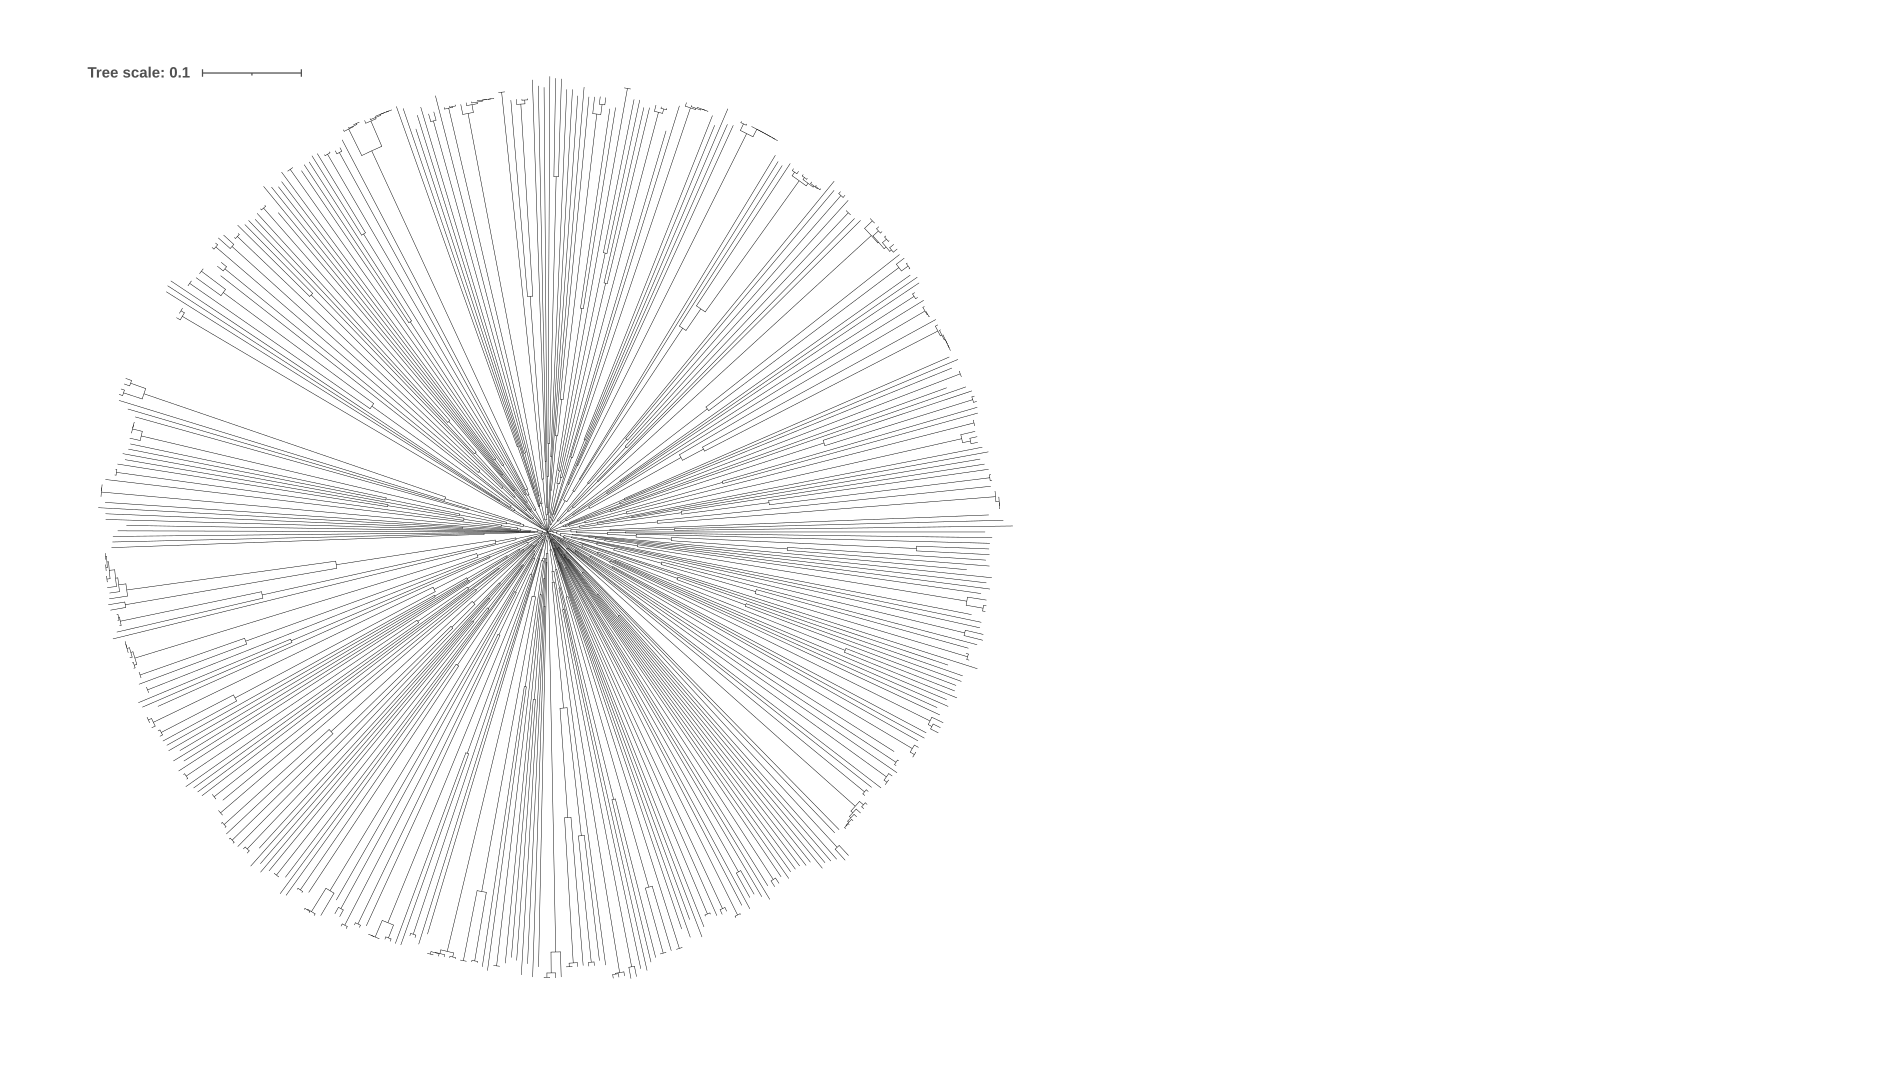
\includegraphics[width=\textwidth]{figures/o-pol-tree.png}
    \caption{Mafft tree of all O-Pol seeds}
    \label{fig:o-pol-seed-tree}
\end{figure}
%https://itol.embl.de/tree/1923813231488581653910690

\begin{figure}[htbp]
    \centering
    \includegraphics[width=\textwidth]{figures/inverting.png}
    \caption{Active sites of inverting CAZy families. The conserved residues of the families are shown on AlphaFold models of representative members of the families.}
    \label{fig:inverting-active-sites}
\end{figure}

\begin{figure}[htbp]
    \centering
    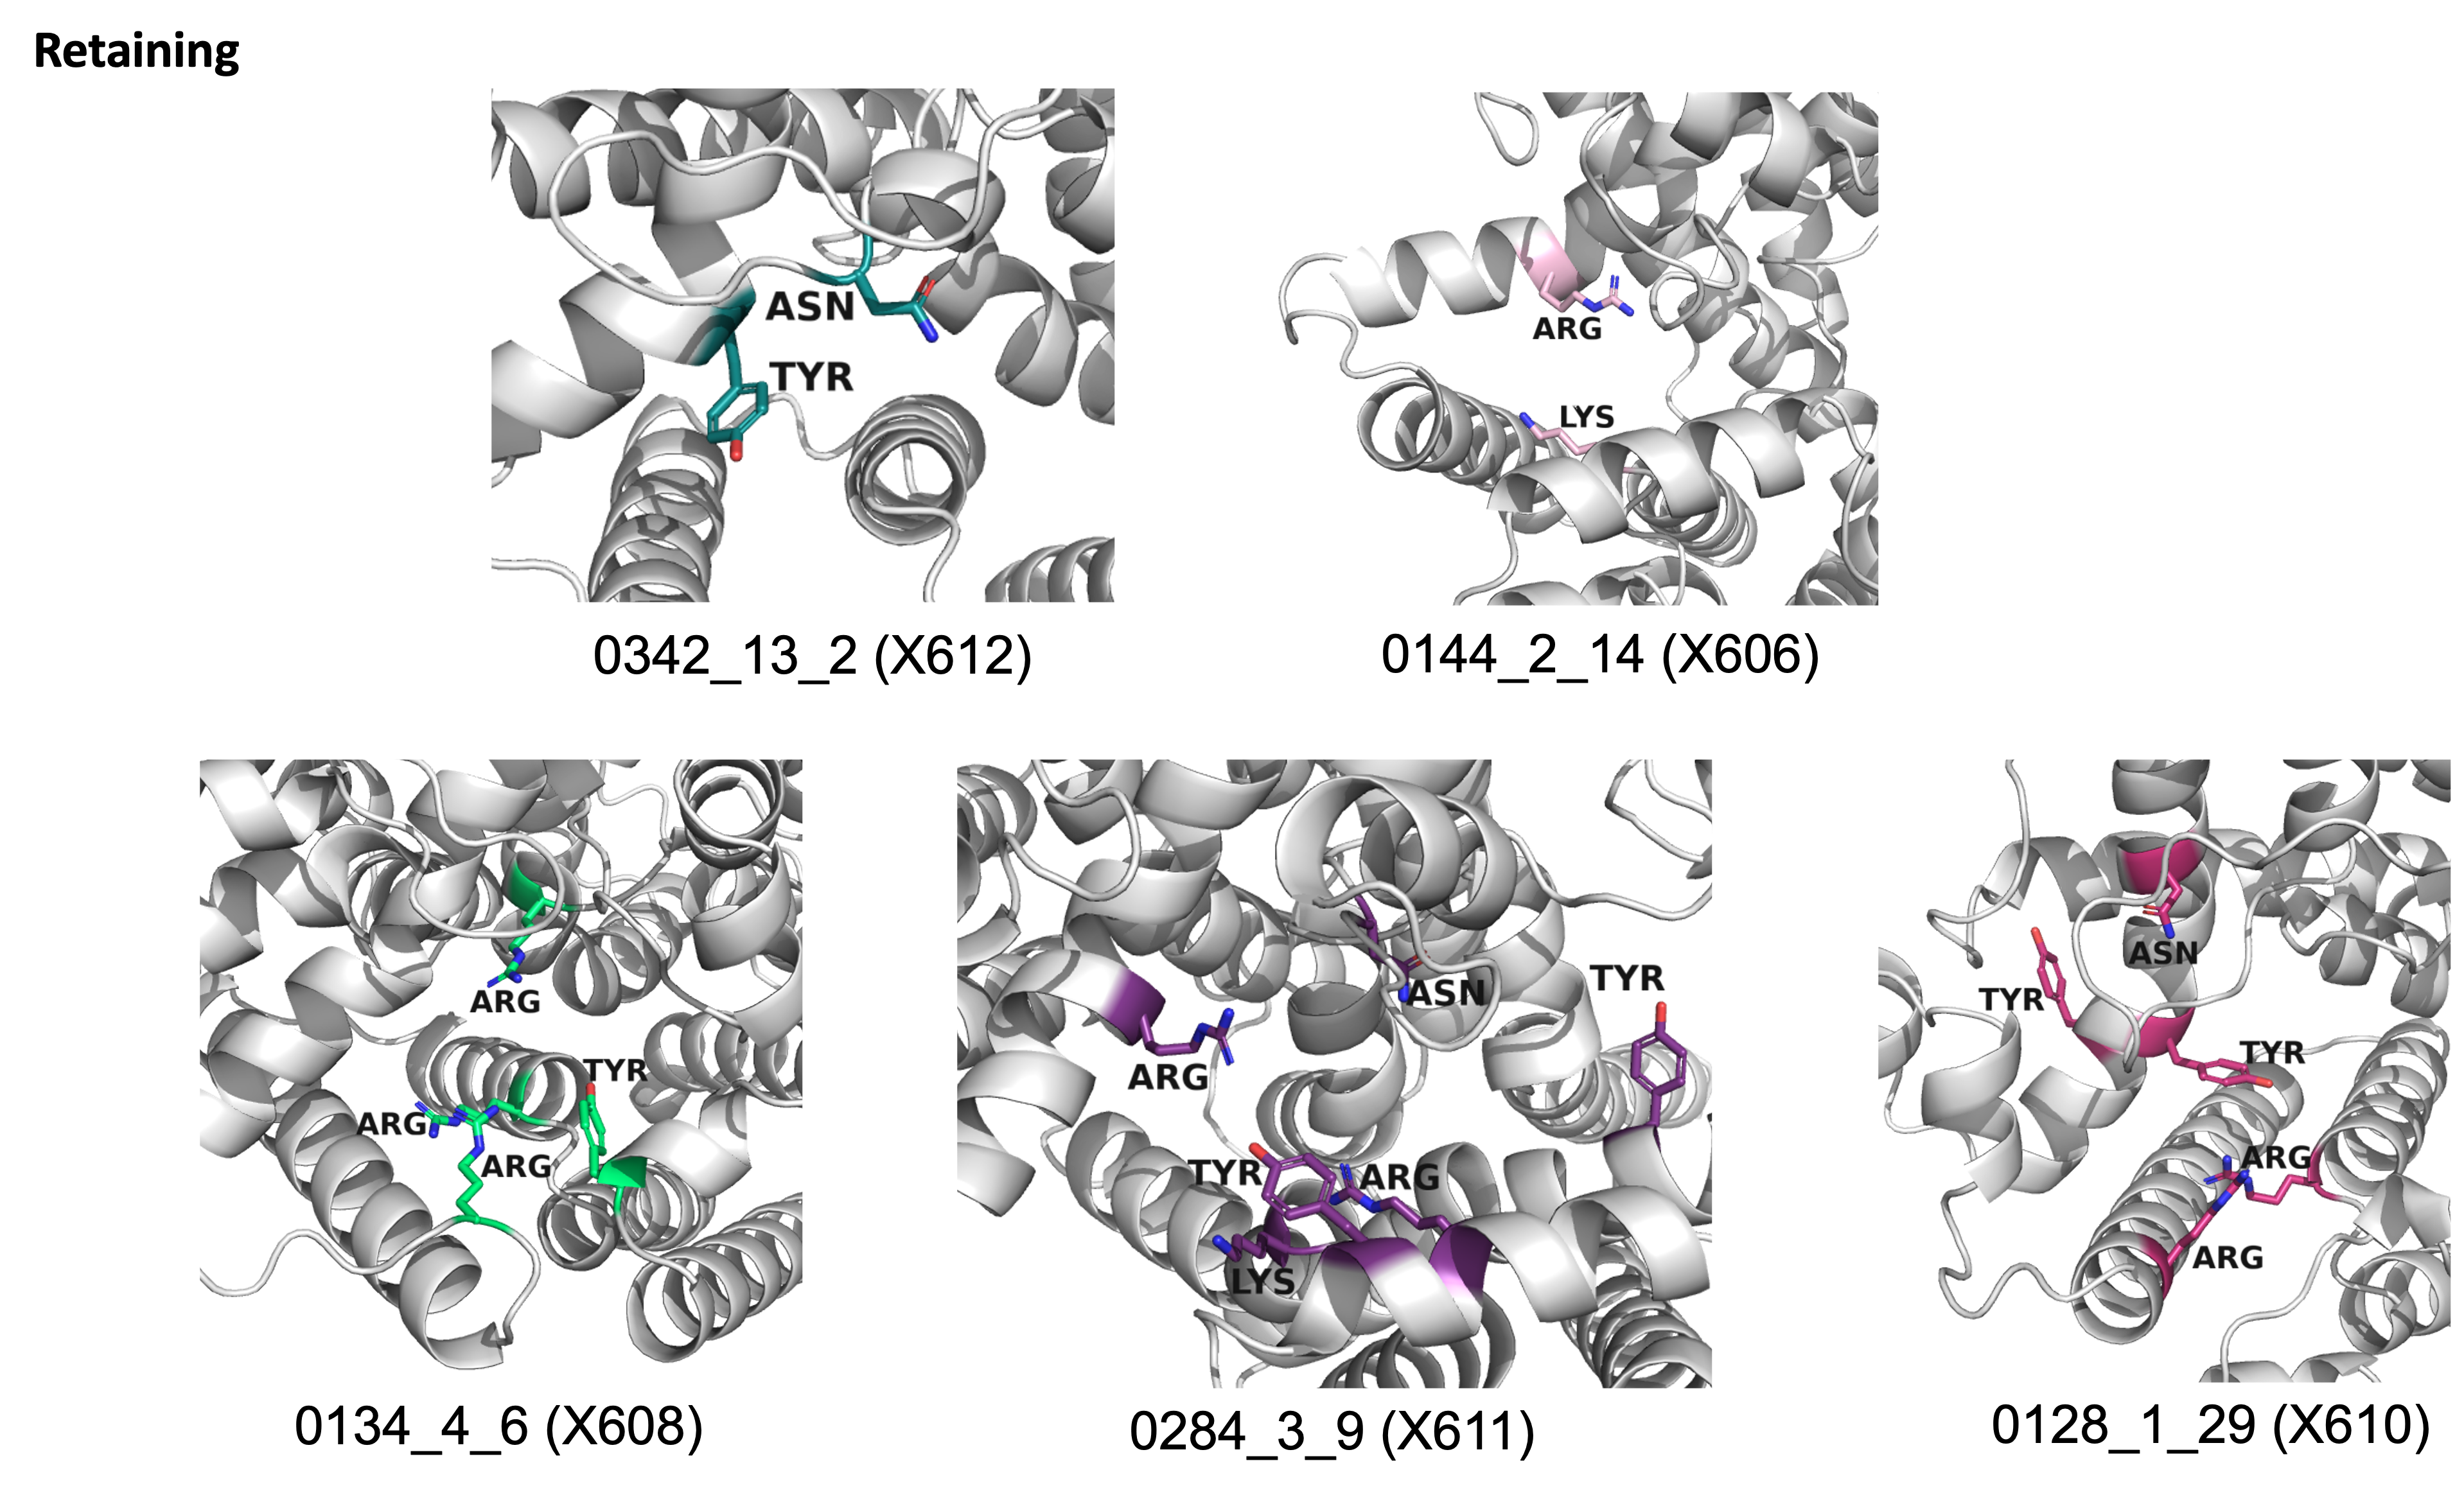
\includegraphics[width=.75\textwidth]{figures/retaining.png}
    \caption{Active sites of retaining CAZy families. The conserved residues of the families are shown on AlphaFold models of representative members of the families.}
    \label{fig:retaining-active-sites}
\end{figure}

\begin{table}[!ht]
    \centering
    \begin{tabular}{|l|l|l|l|}
    \hline
        Family & Number of members & Stereochemistry & Enzyme function \\ \hline
        X571 & 57,278 & Inverting & RodA \\ \hline
        X586 & 4,850 & Retaining & ECA-Pol \\ \hline
        X615 & 16,700 & Inverting & O-lig \\ \hline
        X605 & 704 & Inverting & O-Pol \\ \hline
        X606 & 196 & Retaining & O-Pol \\ \hline
        X607 & 161 & Inverting & O-Pol \\ \hline
        X608 & 184 & Retaining & O-Pol \\ \hline
        X609 & 148 & Inverting & O-Pol \\ \hline
        X610 & 238 & Retaining & O-Pol \\ \hline
        X611 & 260 & Retaining & O-Pol \\ \hline
        X612 & 517 & Retaining & O-Pol \\ \hline
        X613 & 948 & Inverting & O-Pol \\ \hline
        X614 & 159 & Retaining & O-Pol \\ \hline
        X617 & 5,979 & Inverting & O-Pol \\ \hline
    \end{tabular}
    \caption{New CAZy families.}
    \label{tab:families}
\end{table}

\begin{table}[!ht]
    \centering
    \begin{tabular}{|l|l|l|l|l|}
    \hline
        ~ & X571 (SEDS) & X615 (O-Lig) & X586 (ECA-Pol) & Known O-Pol families \\ \hline
        Escherichia coli & 2 & 1 & 1 & 0-1 \\ \hline
        Pseudomonas aeruginosa & 2 & 1 & 0 & 0-2 \\ \hline
        Streptococcus pneumoniae & 2 & 1 & 0 & 0-1 \\ \hline
        Lactiplantibacillus plantarum & 2-3 & 0 & 0 & 0-5 \\ \hline
        Bacteroides fragilis & 2 & 0-1 & 0 & 1-7 \\ \hline
        Bacteroides ovatus & 2 & 0-1 & 0 & 0-4 \\ \hline
        Bacteroides thetaiotaomicron & 2 & 0-4 & 0 & 2-7 \\ \hline
    \end{tabular}
    \caption{Count of members of SEDS, O-Lig and O-Pol families in genomes of different species species.}
    \label{tab:count_members_species}
\end{table}

\begin{table}[!ht]
\begin{tabular}{lllll}
                                       & X571 (SEDS)                                      & X615 (O-Lig)                & X586 (ECA-Pol)            & Known O-Pol families                               \\
\textit{Escherichia coli}              & \cellcolor[HTML]{D2E3FA}{\color[HTML]{000000} 2} & \cellcolor[HTML]{E5EDF8}1   & \cellcolor[HTML]{E5EDF8}1 & \cellcolor[HTML]{E5EDF8}0-1                        \\
\textit{Pseudomonas aeruginosa}        & \cellcolor[HTML]{D2E3FA}{\color[HTML]{000000} 2} & \cellcolor[HTML]{E5EDF8}1   & 0                         & \cellcolor[HTML]{D2E3FA}0-2                        \\
\textit{Streptococcus pneumoniae}      & \cellcolor[HTML]{D2E3FA}{\color[HTML]{000000} 2} & \cellcolor[HTML]{E5EDF8}1   & 0                         & \cellcolor[HTML]{E5EDF8}0-1                        \\
\textit{Lactiplantibacillus plantarum} & \cellcolor[HTML]{BAC1FF}2-3                      & 0                           & 0                         & \cellcolor[HTML]{8A8FF8}0-5                        \\
\textit{Bacteroides fragilis}          & \cellcolor[HTML]{D2E3FA}2                        & \cellcolor[HTML]{E5EDF8}0-1 & 0                         & \cellcolor[HTML]{6B72FA}1-7                        \\
\textit{Bacteroides ovatus}            & \cellcolor[HTML]{D2E3FA}2                        & \cellcolor[HTML]{E5EDF8}0-1 & 0                         & \cellcolor[HTML]{A4A0FF}{\color[HTML]{333333} 0-4} \\
\textit{Bacteroides thetaiotaomicron}  & \cellcolor[HTML]{D2E3FA}2                        & \cellcolor[HTML]{A4A0FF}0-4 & 0                         & \cellcolor[HTML]{6068FA}2-7                       
\end{tabular}
\caption{Count of members of SEDS, O-Lig, ECA-Pol and known O-Pol families in genomes of different species species.}
\label{tab:count_members_species2}
\end{table}

\begin{figure}[htbp]
    \centering
    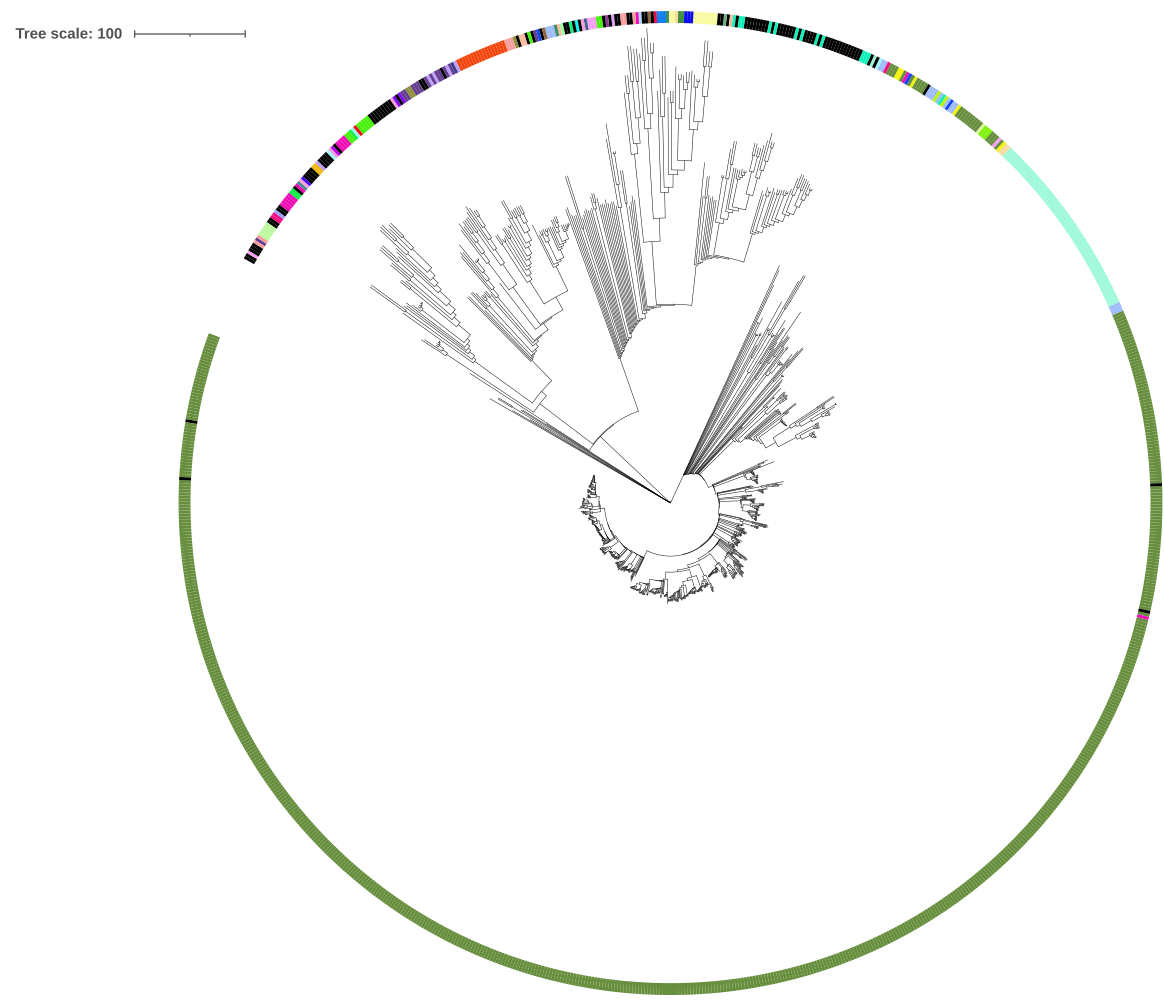
\includegraphics[width=0.6\textwidth]{figures/eca-pol-tree.png}
    \caption{Aclust tree of ECA-Pol sequence space}
    \label{fig:eca-pol-tree}
\end{figure}
%https://itol.embl.de/tree/1923890169486281673015321

Most cell-surface are synthesized via the Wzx/Wzy-dependent pathway in both Gram-positives \cite{paton_streptococcus_2019} and Gram-negatives \cite{islam_synthesis_2014}. In this pathway, the O-antigen repeat units are synthesized on a Und-P carrier the cytoplasmic side of the membrane (inner membrane in Gram-negatives) and flipped to the outside of the membrane by Wzx. O-antigen polymerases (WzyB, O-Pol) then catalyze the polymerization of the repeat units, by transferring the growing polymer to the incoming new repeat units \cite{islam_synthesis_2014}. 

\end{document}